% Problems, Chapter 14: Radiation by Moving Charges
% Jackson, Classical Electrodynamics, 3rd ed.
% Requires: amsmath, amssymb, tikz

\section*{Problems}

\Needspace{5\baselineskip}
\par\bigskip
\noindent\textbf{14.1}\quad Verify by explicit calculation that the Li\'enard--Wiechert expressions for \emph{all} components of $\mathbf{E}$ and $\mathbf{B}$ for a particle moving with constant velocity agree with the ones obtained in the text by means of a Lorentz transformation. Follow the general method at the end of Section 14.1.
\solution

We use Gaussian units throughout this chapter. Let the observation time be
$t$, let $\mathbf r=\mathbf x-\mathbf v t$ point from the \emph{present}
position of the charge, and write $\mathbf R=R\mathbf n$ for the vector
from its retarded position. Uniform motion and $t-t'=R/c$ imply
\[
\mathbf R=\mathbf r+\boldsymbol\beta R,\qquad
\mathbf r=R(\mathbf n-\boldsymbol\beta).
\]
Squaring the first equation gives
$(1-\beta^2)R^2-2(\boldsymbol\beta\cdot\mathbf r)R-r^2=0$.
The positive retarded-distance root is
\[
R=\frac{\boldsymbol\beta\cdot\mathbf r+s}{1-\beta^2},\quad
s=\sqrt{(\boldsymbol\beta\cdot\mathbf r)^2+(1-\beta^2)r^2}
=\sqrt{r^2-|\boldsymbol\beta\times\mathbf r|^2}.
\]
Taking the scalar product of $\mathbf R=\mathbf r+\boldsymbol\beta R$
with $\boldsymbol\beta$ shows
$R(1-\mathbf n\cdot\boldsymbol\beta)
=(1-\beta^2)R-\boldsymbol\beta\cdot\mathbf r=s$.
Since the acceleration term is zero, the Li\'enard--Wiechert fields reduce to
\[
\boxed{\mathbf E=\frac{e(1-\beta^2)\mathbf r}{s^3},\qquad
\mathbf B=\mathbf n\times\mathbf E
=\boldsymbol\beta\times\mathbf E.}
\]
The second equality uses $\mathbf n=\boldsymbol\beta+\mathbf r/R$ and
$\mathbf E\parallel\mathbf r$.

For an explicit component comparison, take $\mathbf v=v\hat{\mathbf z}$,
$z_*=z-vt$, and $D_*=[x^2+y^2+\gamma^2z_*^2]^{3/2}$. Then
\[
(E_x,E_y,E_z)=\frac{e\gamma}{D_*}(x,y,z_*),\qquad
(B_x,B_y,B_z)=\frac{e\gamma\beta}{D_*}(-y,x,0).
\]
In the rest frame $x'=x$, $y'=y$, $z'=\gamma z_*$,
$r'^2=x^2+y^2+\gamma^2z_*^2$, and
$\mathbf E'=e(x',y',z')/r'^3$, $\mathbf B'=0$.
The transformations $E_z=E'_z$, $\mathbf E_\perp=\gamma\mathbf E'_\perp$,
and $\mathbf B=\boldsymbol\beta\times\mathbf E$ reproduce every component
above, including both vanishing longitudinal magnetic and transverse
special cases.

\Needspace{5\baselineskip}
\par\bigskip
\noindent\textbf{14.2}\quad A particle of charge $e$ is moving in nearly uniform nonrelativistic motion. For times near $t=t_{0}$, its vectorial position can be expanded in a Taylor series with fixed vector coefficients multiplying powers of $(t-t_{0})$.
\begin{enumerate}
\item[(a)] Show that, in an inertial frame where the particle is instantaneously at rest at the origin but has a small acceleration $\mathbf{a}$, the Li\'enard--Wiechert electric field, correct to order $1/c^{2}$ inclusive, at that instant is $\mathbf{E}=\mathbf{E}_{v}+\mathbf{E}_{a}$, where the velocity and acceleration fields are
\[
\mathbf{E}_{v}=e\frac{\hat{\mathbf{r}}}{r^{2}}+\frac{e}{2c^{2}r}\,[\mathbf{a}-3\hat{\mathbf{r}}(\hat{\mathbf{r}}\cdot\mathbf{a})];\qquad
\mathbf{E}_{a}=-\frac{e}{c^{2}r}\,[\mathbf{a}-\hat{\mathbf{r}}(\hat{\mathbf{r}}\cdot\mathbf{a})]
\]
and that the total electric field to this order is
\[
\mathbf{E}=e\frac{\hat{\mathbf{r}}}{r^{2}}-\frac{e}{2c^{2}r}\,[\mathbf{a}+\hat{\mathbf{r}}(\hat{\mathbf{r}}\cdot\mathbf{a})]
\]
The unit vector $\hat{\mathbf{r}}$ points from the origin to the observation point and $r$ is the magnitude of the distance. Comment on the $r$ dependences of the velocity and acceleration fields. Where is the expansion likely to be valid?
\item[(b)] What is the result for the instantaneous magnetic induction $\mathbf{B}$ to the same order? Comment.
\item[(c)] Show that the $1/c^{2}$ term in the electric field has zero divergence and that the curl of the electric field is $\nabla\times\mathbf{E}=e(\hat{\mathbf{r}}\times\mathbf{a})/c^{2}r^{2}$. From Faraday's law, find the magnetic induction $\mathbf{B}$ at times near $t=0$. Compare with the familiar elementary expression.
\end{enumerate}
\solution

Set the instant in question to $t=0$, so
$\mathbf r_q(t')=\tfrac12\mathbf a t'^2+O(t'^3)$ and
$\boldsymbol\beta(t')=\mathbf a t'/c+O(t'^2/c)$.
All expansions below hold at fixed $r$ as $c$ becomes large, retaining
terms through $c^{-2}$.

\textbf{(a)} The retarded equation gives
$t'=-r/c+O(c^{-3})$. Consequently
\[
\mathbf r_q(t')=\frac{r^2\mathbf a}{2c^2}+O(c^{-3}),\quad
\boldsymbol\beta_{\rm ret}=-\frac{r\mathbf a}{c^2}+O(c^{-3}),
\]
\[
R=r-\frac{r^2\hat{\mathbf r}\cdot\mathbf a}{2c^2}+O(c^{-3}),\quad
\mathbf n=\hat{\mathbf r}-\frac r{2c^2}
[\mathbf a-\hat{\mathbf r}(\hat{\mathbf r}\cdot\mathbf a)]+O(c^{-3}).
\]
Put $A=\hat{\mathbf r}\cdot\mathbf a$ and
$\kappa=1-\mathbf n\cdot\boldsymbol\beta$. The factors in the velocity
field become
\[
\kappa^{-3}=1-3rA/c^2+O(c^{-3}),\quad
R^{-2}=r^{-2}(1+rA/c^2)+O(c^{-3}),\quad
\mathbf n-\boldsymbol\beta=\hat{\mathbf r}
+\frac r{2c^2}(\mathbf a+A\hat{\mathbf r})+O(c^{-3}).
\]
Also $1-\beta^2=1+O(c^{-4})$. Multiplication gives
\[
\mathbf E_v=\frac e{r^2}\left[
\hat{\mathbf r}+\frac r{2c^2}(\mathbf a+A\hat{\mathbf r})
-\frac{2rA}{c^2}\hat{\mathbf r}\right]
=\frac{e\hat{\mathbf r}}{r^2}
+\frac e{2c^2r}(\mathbf a-3A\hat{\mathbf r}).
\]
In the acceleration term it suffices at this order to set
$R=r$, $\mathbf n=\hat{\mathbf r}$, $\boldsymbol\beta=0$:
\[
\mathbf E_a=\frac e{c^2r}\hat{\mathbf r}\times
(\hat{\mathbf r}\times\mathbf a)
=-\frac e{c^2r}(\mathbf a-A\hat{\mathbf r}).
\]
Adding proves $\mathbf E=e\hat{\mathbf r}/r^2-
 e(\mathbf a+A\hat{\mathbf r})/(2c^2r)$.
The exact velocity and acceleration fields scale as $R^{-2}$ and $R^{-1}$
when written in retarded variables. Expanding the retarded position and
velocity about the present instant introduces $r^{-1}$ terms into the
former too. This is a local slow-motion expansion, requiring
$ar/c^2\ll1$ and higher terms such as $|\dot{\mathbf a}|r^2/c^3\ll1$;
it cannot be extended without restriction to the distant radiation zone.

\textbf{(b)} Use the retarded $\mathbf n$, not $\hat{\mathbf r}$, in
$\mathbf B=\mathbf n\times\mathbf E$. The two contributions are
\[
\hat{\mathbf r}\times\delta\mathbf E
=-\frac e{2c^2r}\hat{\mathbf r}\times\mathbf a,\qquad
\delta\mathbf n\times\frac{e\hat{\mathbf r}}{r^2}
=+\frac e{2c^2r}\hat{\mathbf r}\times\mathbf a.
\]
They cancel: $\boxed{\mathbf B(\mathbf x,0)=0+O(c^{-3})}$.
An instantaneous rest frame does not remove the acceleration electric
field, but it does remove the magnetic field through this order.

\textbf{(c)} Write the correction as
$\delta\mathbf E=-e[\mathbf a/r+
\mathbf r(\mathbf a\cdot\mathbf r)/r^3]/(2c^2)$.
For $r>0$,
\[
\nabla\cdot(\mathbf a/r)=-\frac{\mathbf a\cdot\mathbf r}{r^3},\qquad
\nabla\cdot\left[\frac{\mathbf r(\mathbf a\cdot\mathbf r)}{r^3}\right]
=\frac{\mathbf a\cdot\mathbf r}{r^3},
\]
so its divergence is zero. There is no added delta function at the origin
because its flux through a shrinking sphere tends to zero.
Furthermore
\[
\nabla\times(\mathbf a/r)=-\frac{\hat{\mathbf r}\times\mathbf a}{r^2},
\quad
\nabla\times\left[\frac{\mathbf r(\mathbf a\cdot\mathbf r)}{r^3}\right]
=-\frac{\hat{\mathbf r}\times\mathbf a}{r^2}.
\]
Thus $\nabla\times\mathbf E=e\hat{\mathbf r}\times\mathbf a/(c^2r^2)$.
Faraday's law gives $\partial_t\mathbf B=e\mathbf a\times
\hat{\mathbf r}/(cr^2)$, and integration about $t=0$ yields
\[
\boxed{\mathbf B(\mathbf x,t)=\frac{e}{cr^2}
(t\mathbf a)\times\hat{\mathbf r}+\cdots
=\frac{e\mathbf v(t)\times\hat{\mathbf r}}{cr^2}+\cdots.}
\]
This is precisely the elementary nonrelativistic moving-charge field.

\Needspace{5\baselineskip}
\par\bigskip
\noindent\textbf{14.3}\quad The Heaviside--Feynman expression for the electric field of a particle of charge $e$ in arbitrary motion, an alternative to the Li\'enard--Wiechert expression (14.14), is
\[
\mathbf{E}=e\left[\frac{\mathbf{n}}{R^{2}}\right]_{\mathrm{ret}}+e\left[\frac{R}{c}\right]_{\mathrm{ret}}\frac{d}{dt}\left[\frac{\mathbf{n}}{R^{2}}\right]_{\mathrm{ret}}+e\frac{d^{2}}{c^{2}dt^{2}}\,[\mathbf{n}]_{\mathrm{ret}}
\]
where the time derivatives are with respect to the time at the observation point. The magnetic field is given by (14.13).

Using the fact that the retarded time is $t'=t-R(t')/c$ and that, as a result,
\[
\frac{dt}{dt'}=1-\boldsymbol{\beta}(t')\cdot\mathbf{n}(t')
\]
show that the form above yields (14.14) when the time differentiations are performed.
\solution

All unbracketed quantities in this derivation are evaluated at $t'$.
Define $b=\mathbf n\cdot\boldsymbol\beta$, $\kappa=1-b$, and
$\mathbf u=b\mathbf n-\boldsymbol\beta$. At a fixed observation point,
\[
\frac d{dt}=\kappa^{-1}\frac d{dt'},\quad
\dot R=-cb,\quad \dot{\mathbf n}=\frac cR\mathbf u,\quad
\dot b=\frac cR(b^2-\beta^2)+\mathbf n\cdot\dot{\boldsymbol\beta},
\]
where a dot here means $d/dt'$. The first differentiated expression is
\[
\frac d{dt}\frac{\mathbf n}{R^2}
=\frac c{\kappa R^3}(3b\mathbf n-\boldsymbol\beta).
\]
For the second, differentiate $d\mathbf n/dt=c\mathbf u/(R\kappa)$
and use $\dot{\mathbf u}=\dot b\mathbf n+cb\mathbf u/R-
\dot{\boldsymbol\beta}$. This gives
\[
\frac{d^2\mathbf n}{dt^2}
=\frac c{R\kappa^2}\left[
\dot b\mathbf n-\dot{\boldsymbol\beta}
+\left(\frac{2cb}R+\frac{\dot b}{\kappa}\right)\mathbf u\right].
\]
Substitute these in the proposed field and split $\dot b$ into its
velocity and acceleration parts. The coefficient of $\mathbf n/R^2$
has numerator
\[
(1+2b)\kappa^2+(b^2-\beta^2)\kappa
+b[2b\kappa+b^2-\beta^2]=1-\beta^2,
\]
and that of $\boldsymbol\beta/R^2$ has numerator
$-\kappa^2-2b\kappa-b^2+\beta^2=-(1-\beta^2)$, both over $\kappa^3$.
Writing $q=\mathbf n\cdot\dot{\boldsymbol\beta}$, the remaining terms
are
\[
\frac e{cR\kappa^3}
[q(\mathbf n-\boldsymbol\beta)-\kappa\dot{\boldsymbol\beta}]
=\frac e{cR\kappa^3}\mathbf n\times
[(\mathbf n-\boldsymbol\beta)\times\dot{\boldsymbol\beta}].
\]
Therefore
\[
\boxed{\mathbf E=e\left[
\frac{(1-\beta^2)(\mathbf n-\boldsymbol\beta)}{\kappa^3R^2}
+\frac{\mathbf n\times[(\mathbf n-\boldsymbol\beta)
\times\dot{\boldsymbol\beta}]}{c\kappa^3R}\right]_{\rm ret},}
\]
which is (14.14), with $\mathbf B=\mathbf n\times\mathbf E$.
The factors of $\kappa^{-1}$ from observation-time differentiation are
essential to the result.

\Needspace{5\baselineskip}
\par\bigskip
\noindent\textbf{14.4}\quad Using the Li\'enard--Wiechert fields, discuss the time-averaged power radiated per unit solid angle in nonrelativistic motion of a particle with charge $e$, moving
\begin{enumerate}
\item[(a)] along the $z$ axis with instantaneous position $z(t)=a\cos\omega_{0}t$,
\item[(b)] in a circle of radius $R$ in the $x$-$y$ plane with constant angular frequency $\omega_{0}$.
\end{enumerate}
Sketch the angular distribution of the radiation and determine the total power radiated in each case.
\solution

To leading nonrelativistic order the acceleration field is
$\mathbf E_a=e\mathbf n\times(\mathbf n\times\mathbf a)/(c^2R)$,
$\mathbf B_a=\mathbf n\times\mathbf E_a$. The Gaussian Poynting flux
$c|\mathbf E_a|^2/(4\pi)$ therefore gives
\[
\frac{d\overline P}{d\Omega}
=\frac{e^2}{4\pi c^3}
\left[\overline{a^2}-\overline{(\mathbf n\cdot\mathbf a)^2}\right].
\]
At this order the distinction between source-time and arrival-time
averages is beyond the retained accuracy.

\textbf{(a)} For $z=a\cos\omega_0t$,
$\mathbf a=-a\omega_0^2\cos\omega_0t\,\hat{\mathbf z}$.
Using $\overline{\cos^2\omega_0t}=1/2$ gives
\[
\boxed{\frac{d\overline P}{d\Omega}
=\frac{e^2a^2\omega_0^4}{8\pi c^3}\sin^2\theta,
\qquad \overline P=\frac{e^2a^2\omega_0^4}{3c^3}.}
\]
The angular integral is $2\pi\int_{-1}^1(1-u^2)du=8\pi/3$.

\textbf{(b)} For circular motion,
$\mathbf a=-R\omega_0^2(\hat{\mathbf x}\cos\omega_0t+
\hat{\mathbf y}\sin\omega_0t)$.
Here $\overline{a^2}=R^2\omega_0^4$ and
$\overline{(\mathbf n\cdot\mathbf a)^2}=
R^2\omega_0^4\sin^2\theta/2$. Hence
\[
\boxed{\frac{d\overline P}{d\Omega}
=\frac{e^2R^2\omega_0^4}{8\pi c^3}(1+\cos^2\theta),
\qquad \overline P=\frac{2e^2R^2\omega_0^4}{3c^3}.}
\]
This time $2\pi\int_{-1}^1(1+u^2)du=16\pi/3$.
The meridional polar plots below use normalized intensity as radius;
rotation about $z$ gives the full distributions.
\begin{center}% Generated by supplementary/check_ch14.py
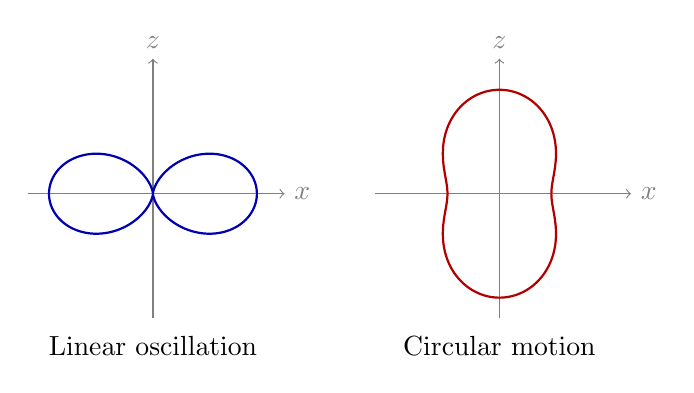
\begin{tikzpicture}[scale=.88]
\begin{scope}[xshift=0cm]
\draw[->,gray] (-1.8,0)--(1.9,0) node[right]{$x$};
\draw[->,gray] (0,-1.8)--(0,1.95) node[above]{$z$};
\draw[blue!70!black,thick] plot coordinates {(0.00000,0.00000) (0.00001,0.00046) (0.00006,0.00183) (0.00022,0.00410) (0.00051,0.00728) (0.00099,0.01135) (0.00171,0.01630) (0.00272,0.02211) (0.00404,0.02877) (0.00574,0.03626) (0.00785,0.04454) (0.01042,0.05361) (0.01348,0.06342) (0.01707,0.07396) (0.02124,0.08518) (0.02601,0.09706) (0.03141,0.10955) (0.03749,0.12262) (0.04426,0.13623) (0.05176,0.15033) (0.06001,0.16488) (0.06904,0.17985) (0.07885,0.19517) (0.08948,0.21080) (0.10093,0.22670) (0.11322,0.24281) (0.12636,0.25908) (0.14036,0.27546) (0.15521,0.29191) (0.17092,0.30836) (0.18750,0.32476) (0.20493,0.34106) (0.22321,0.35722) (0.24234,0.37316) (0.26229,0.38886) (0.28305,0.40424) (0.30461,0.41926) (0.32695,0.43388) (0.35004,0.44803) (0.37386,0.46168) (0.39838,0.47477) (0.42356,0.48726) (0.44939,0.49910) (0.47582,0.51025) (0.50281,0.52068) (0.53033,0.53033) (0.55833,0.53918) (0.58678,0.54718) (0.61562,0.55431) (0.64481,0.56052) (0.67430,0.56580) (0.70404,0.57012) (0.73399,0.57345) (0.76408,0.57577) (0.79426,0.57707) (0.82449,0.57731) (0.85470,0.57650) (0.88484,0.57462) (0.91486,0.57167) (0.94469,0.56763) (0.97428,0.56250) (1.00357,0.55629) (1.03251,0.54900) (1.06105,0.54063) (1.08911,0.53119) (1.11665,0.52070) (1.14362,0.50917) (1.16996,0.49662) (1.19561,0.48306) (1.22052,0.46852) (1.24465,0.45302) (1.26795,0.43659) (1.29036,0.41926) (1.31184,0.40107) (1.33234,0.38204) (1.35183,0.36222) (1.37026,0.34164) (1.38760,0.32035) (1.40380,0.29839) (1.41883,0.27579) (1.43267,0.25262) (1.44528,0.22891) (1.45663,0.20472) (1.46671,0.18009) (1.47548,0.15508) (1.48294,0.12974) (1.48906,0.10413) (1.49384,0.07829) (1.49726,0.05229) (1.49931,0.02617) (1.50000,0.00000) (1.49931,-0.02617) (1.49726,-0.05229) (1.49384,-0.07829) (1.48906,-0.10413) (1.48294,-0.12974) (1.47548,-0.15508) (1.46671,-0.18009) (1.45663,-0.20472) (1.44528,-0.22891) (1.43267,-0.25262) (1.41883,-0.27579) (1.40380,-0.29839) (1.38760,-0.32035) (1.37026,-0.34164) (1.35183,-0.36222) (1.33234,-0.38204) (1.31184,-0.40107) (1.29036,-0.41926) (1.26795,-0.43659) (1.24465,-0.45302) (1.22052,-0.46852) (1.19561,-0.48306) (1.16996,-0.49662) (1.14362,-0.50917) (1.11665,-0.52070) (1.08911,-0.53119) (1.06105,-0.54063) (1.03251,-0.54900) (1.00357,-0.55629) (0.97428,-0.56250) (0.94469,-0.56763) (0.91486,-0.57167) (0.88484,-0.57462) (0.85470,-0.57650) (0.82449,-0.57731) (0.79426,-0.57707) (0.76408,-0.57577) (0.73399,-0.57345) (0.70404,-0.57012) (0.67430,-0.56580) (0.64481,-0.56052) (0.61562,-0.55431) (0.58678,-0.54718) (0.55833,-0.53918) (0.53033,-0.53033) (0.50281,-0.52068) (0.47582,-0.51025) (0.44939,-0.49910) (0.42356,-0.48726) (0.39838,-0.47477) (0.37386,-0.46168) (0.35004,-0.44803) (0.32695,-0.43388) (0.30461,-0.41926) (0.28305,-0.40424) (0.26229,-0.38886) (0.24234,-0.37316) (0.22321,-0.35722) (0.20493,-0.34106) (0.18750,-0.32476) (0.17092,-0.30836) (0.15521,-0.29191) (0.14036,-0.27546) (0.12636,-0.25908) (0.11322,-0.24281) (0.10093,-0.22670) (0.08948,-0.21080) (0.07885,-0.19517) (0.06904,-0.17985) (0.06001,-0.16488) (0.05176,-0.15033) (0.04426,-0.13623) (0.03749,-0.12262) (0.03141,-0.10955) (0.02601,-0.09706) (0.02124,-0.08518) (0.01707,-0.07396) (0.01348,-0.06342) (0.01042,-0.05361) (0.00785,-0.04454) (0.00574,-0.03626) (0.00404,-0.02877) (0.00272,-0.02211) (0.00171,-0.01630) (0.00099,-0.01135) (0.00051,-0.00728) (0.00022,-0.00410) (0.00006,-0.00183) (0.00001,-0.00046) (0.00000,-0.00000) (-0.00001,-0.00046) (-0.00006,-0.00183) (-0.00022,-0.00410) (-0.00051,-0.00728) (-0.00099,-0.01135) (-0.00171,-0.01630) (-0.00272,-0.02211) (-0.00404,-0.02877) (-0.00574,-0.03626) (-0.00785,-0.04454) (-0.01042,-0.05361) (-0.01348,-0.06342) (-0.01707,-0.07396) (-0.02124,-0.08518) (-0.02601,-0.09706) (-0.03141,-0.10955) (-0.03749,-0.12262) (-0.04426,-0.13623) (-0.05176,-0.15033) (-0.06001,-0.16488) (-0.06904,-0.17985) (-0.07885,-0.19517) (-0.08948,-0.21080) (-0.10093,-0.22670) (-0.11322,-0.24281) (-0.12636,-0.25908) (-0.14036,-0.27546) (-0.15521,-0.29191) (-0.17092,-0.30836) (-0.18750,-0.32476) (-0.20493,-0.34106) (-0.22321,-0.35722) (-0.24234,-0.37316) (-0.26229,-0.38886) (-0.28305,-0.40424) (-0.30461,-0.41926) (-0.32695,-0.43388) (-0.35004,-0.44803) (-0.37386,-0.46168) (-0.39838,-0.47477) (-0.42356,-0.48726) (-0.44939,-0.49910) (-0.47582,-0.51025) (-0.50281,-0.52068) (-0.53033,-0.53033) (-0.55833,-0.53918) (-0.58678,-0.54718) (-0.61562,-0.55431) (-0.64481,-0.56052) (-0.67430,-0.56580) (-0.70404,-0.57012) (-0.73399,-0.57345) (-0.76408,-0.57577) (-0.79426,-0.57707) (-0.82449,-0.57731) (-0.85470,-0.57650) (-0.88484,-0.57462) (-0.91486,-0.57167) (-0.94469,-0.56763) (-0.97428,-0.56250) (-1.00357,-0.55629) (-1.03251,-0.54900) (-1.06105,-0.54063) (-1.08911,-0.53119) (-1.11665,-0.52070) (-1.14362,-0.50917) (-1.16996,-0.49662) (-1.19561,-0.48306) (-1.22052,-0.46852) (-1.24465,-0.45302) (-1.26795,-0.43659) (-1.29036,-0.41926) (-1.31184,-0.40107) (-1.33234,-0.38204) (-1.35183,-0.36222) (-1.37026,-0.34164) (-1.38760,-0.32035) (-1.40380,-0.29839) (-1.41883,-0.27579) (-1.43267,-0.25262) (-1.44528,-0.22891) (-1.45663,-0.20472) (-1.46671,-0.18009) (-1.47548,-0.15508) (-1.48294,-0.12974) (-1.48906,-0.10413) (-1.49384,-0.07829) (-1.49726,-0.05229) (-1.49931,-0.02617) (-1.50000,-0.00000) (-1.49931,0.02617) (-1.49726,0.05229) (-1.49384,0.07829) (-1.48906,0.10413) (-1.48294,0.12974) (-1.47548,0.15508) (-1.46671,0.18009) (-1.45663,0.20472) (-1.44528,0.22891) (-1.43267,0.25262) (-1.41883,0.27579) (-1.40380,0.29839) (-1.38760,0.32035) (-1.37026,0.34164) (-1.35183,0.36222) (-1.33234,0.38204) (-1.31184,0.40107) (-1.29036,0.41926) (-1.26795,0.43659) (-1.24465,0.45302) (-1.22052,0.46852) (-1.19561,0.48306) (-1.16996,0.49662) (-1.14362,0.50917) (-1.11665,0.52070) (-1.08911,0.53119) (-1.06105,0.54063) (-1.03251,0.54900) (-1.00357,0.55629) (-0.97428,0.56250) (-0.94469,0.56763) (-0.91486,0.57167) (-0.88484,0.57462) (-0.85470,0.57650) (-0.82449,0.57731) (-0.79426,0.57707) (-0.76408,0.57577) (-0.73399,0.57345) (-0.70404,0.57012) (-0.67430,0.56580) (-0.64481,0.56052) (-0.61562,0.55431) (-0.58678,0.54718) (-0.55833,0.53918) (-0.53033,0.53033) (-0.50281,0.52068) (-0.47582,0.51025) (-0.44939,0.49910) (-0.42356,0.48726) (-0.39838,0.47477) (-0.37386,0.46168) (-0.35004,0.44803) (-0.32695,0.43388) (-0.30461,0.41926) (-0.28305,0.40424) (-0.26229,0.38886) (-0.24234,0.37316) (-0.22321,0.35722) (-0.20493,0.34106) (-0.18750,0.32476) (-0.17092,0.30836) (-0.15521,0.29191) (-0.14036,0.27546) (-0.12636,0.25908) (-0.11322,0.24281) (-0.10093,0.22670) (-0.08948,0.21080) (-0.07885,0.19517) (-0.06904,0.17985) (-0.06001,0.16488) (-0.05176,0.15033) (-0.04426,0.13623) (-0.03749,0.12262) (-0.03141,0.10955) (-0.02601,0.09706) (-0.02124,0.08518) (-0.01707,0.07396) (-0.01348,0.06342) (-0.01042,0.05361) (-0.00785,0.04454) (-0.00574,0.03626) (-0.00404,0.02877) (-0.00272,0.02211) (-0.00171,0.01630) (-0.00099,0.01135) (-0.00051,0.00728) (-0.00022,0.00410) (-0.00006,0.00183) (-0.00001,0.00046) (-0.00000,0.00000)};
\node at (0,-2.2) {Linear oscillation};
\end{scope}
\begin{scope}[xshift=5cm]
\draw[->,gray] (-1.8,0)--(1.9,0) node[right]{$x$};
\draw[->,gray] (0,-1.8)--(0,1.95) node[above]{$z$};
\draw[red!70!black,thick] plot coordinates {(0.00000,1.50000) (0.02617,1.49954) (0.05232,1.49817) (0.07840,1.49589) (0.10438,1.49271) (0.13024,1.48862) (0.15594,1.48363) (0.18145,1.47776) (0.20674,1.47102) (0.23178,1.46340) (0.25655,1.45494) (0.28100,1.44564) (0.30513,1.43551) (0.32889,1.42458) (0.35226,1.41285) (0.37523,1.40036) (0.39775,1.38712) (0.41981,1.37315) (0.44139,1.35847) (0.46247,1.34311) (0.48302,1.32710) (0.50303,1.31045) (0.52248,1.29319) (0.54136,1.27536) (0.55964,1.25697) (0.57732,1.23806) (0.59438,1.21865) (0.61081,1.19878) (0.62660,1.17847) (0.64175,1.15775) (0.65625,1.13666) (0.67009,1.11522) (0.68327,1.09346) (0.69579,1.07142) (0.70765,1.04913) (0.71884,1.02661) (0.72937,1.00389) (0.73925,0.98102) (0.74847,0.95800) (0.75705,0.93488) (0.76499,0.91168) (0.77231,0.88844) (0.77900,0.86517) (0.78509,0.84190) (0.79058,0.81867) (0.79550,0.79550) (0.79984,0.77240) (0.80364,0.74941) (0.80691,0.72654) (0.80966,0.70383) (0.81192,0.68128) (0.81370,0.65892) (0.81502,0.63677) (0.81591,0.61484) (0.81639,0.59315) (0.81648,0.57171) (0.81621,0.55054) (0.81559,0.52965) (0.81464,0.50905) (0.81341,0.48874) (0.81190,0.46875) (0.81014,0.44907) (0.80816,0.42971) (0.80599,0.41067) (0.80364,0.39196) (0.80113,0.37358) (0.79851,0.35552) (0.79578,0.33779) (0.79297,0.32038) (0.79011,0.30329) (0.78721,0.28652) (0.78430,0.27006) (0.78141,0.25389) (0.77854,0.23802) (0.77572,0.22243) (0.77297,0.20712) (0.77031,0.19206) (0.76776,0.17725) (0.76532,0.16267) (0.76302,0.14832) (0.76088,0.13416) (0.75889,0.12020) (0.75709,0.10640) (0.75547,0.09276) (0.75404,0.07925) (0.75282,0.06586) (0.75181,0.05257) (0.75102,0.03936) (0.75046,0.02621) (0.75011,0.01309) (0.75000,0.00000) (0.75011,-0.01309) (0.75046,-0.02621) (0.75102,-0.03936) (0.75181,-0.05257) (0.75282,-0.06586) (0.75404,-0.07925) (0.75547,-0.09276) (0.75709,-0.10640) (0.75889,-0.12020) (0.76088,-0.13416) (0.76302,-0.14832) (0.76532,-0.16267) (0.76776,-0.17725) (0.77031,-0.19206) (0.77297,-0.20712) (0.77572,-0.22243) (0.77854,-0.23802) (0.78141,-0.25389) (0.78430,-0.27006) (0.78721,-0.28652) (0.79011,-0.30329) (0.79297,-0.32038) (0.79578,-0.33779) (0.79851,-0.35552) (0.80113,-0.37358) (0.80364,-0.39196) (0.80599,-0.41067) (0.80816,-0.42971) (0.81014,-0.44907) (0.81190,-0.46875) (0.81341,-0.48874) (0.81464,-0.50905) (0.81559,-0.52965) (0.81621,-0.55054) (0.81648,-0.57171) (0.81639,-0.59315) (0.81591,-0.61484) (0.81502,-0.63677) (0.81370,-0.65892) (0.81192,-0.68128) (0.80966,-0.70383) (0.80691,-0.72654) (0.80364,-0.74941) (0.79984,-0.77240) (0.79550,-0.79550) (0.79058,-0.81867) (0.78509,-0.84190) (0.77900,-0.86517) (0.77231,-0.88844) (0.76499,-0.91168) (0.75705,-0.93488) (0.74847,-0.95800) (0.73925,-0.98102) (0.72937,-1.00389) (0.71884,-1.02661) (0.70765,-1.04913) (0.69579,-1.07142) (0.68327,-1.09346) (0.67009,-1.11522) (0.65625,-1.13666) (0.64175,-1.15775) (0.62660,-1.17847) (0.61081,-1.19878) (0.59438,-1.21865) (0.57732,-1.23806) (0.55964,-1.25697) (0.54136,-1.27536) (0.52248,-1.29319) (0.50303,-1.31045) (0.48302,-1.32710) (0.46247,-1.34311) (0.44139,-1.35847) (0.41981,-1.37315) (0.39775,-1.38712) (0.37523,-1.40036) (0.35226,-1.41285) (0.32889,-1.42458) (0.30513,-1.43551) (0.28100,-1.44564) (0.25655,-1.45494) (0.23178,-1.46340) (0.20674,-1.47102) (0.18145,-1.47776) (0.15594,-1.48363) (0.13024,-1.48862) (0.10438,-1.49271) (0.07840,-1.49589) (0.05232,-1.49817) (0.02617,-1.49954) (0.00000,-1.50000) (-0.02617,-1.49954) (-0.05232,-1.49817) (-0.07840,-1.49589) (-0.10438,-1.49271) (-0.13024,-1.48862) (-0.15594,-1.48363) (-0.18145,-1.47776) (-0.20674,-1.47102) (-0.23178,-1.46340) (-0.25655,-1.45494) (-0.28100,-1.44564) (-0.30513,-1.43551) (-0.32889,-1.42458) (-0.35226,-1.41285) (-0.37523,-1.40036) (-0.39775,-1.38712) (-0.41981,-1.37315) (-0.44139,-1.35847) (-0.46247,-1.34311) (-0.48302,-1.32710) (-0.50303,-1.31045) (-0.52248,-1.29319) (-0.54136,-1.27536) (-0.55964,-1.25697) (-0.57732,-1.23806) (-0.59438,-1.21865) (-0.61081,-1.19878) (-0.62660,-1.17847) (-0.64175,-1.15775) (-0.65625,-1.13666) (-0.67009,-1.11522) (-0.68327,-1.09346) (-0.69579,-1.07142) (-0.70765,-1.04913) (-0.71884,-1.02661) (-0.72937,-1.00389) (-0.73925,-0.98102) (-0.74847,-0.95800) (-0.75705,-0.93488) (-0.76499,-0.91168) (-0.77231,-0.88844) (-0.77900,-0.86517) (-0.78509,-0.84190) (-0.79058,-0.81867) (-0.79550,-0.79550) (-0.79984,-0.77240) (-0.80364,-0.74941) (-0.80691,-0.72654) (-0.80966,-0.70383) (-0.81192,-0.68128) (-0.81370,-0.65892) (-0.81502,-0.63677) (-0.81591,-0.61484) (-0.81639,-0.59315) (-0.81648,-0.57171) (-0.81621,-0.55054) (-0.81559,-0.52965) (-0.81464,-0.50905) (-0.81341,-0.48874) (-0.81190,-0.46875) (-0.81014,-0.44907) (-0.80816,-0.42971) (-0.80599,-0.41067) (-0.80364,-0.39196) (-0.80113,-0.37358) (-0.79851,-0.35552) (-0.79578,-0.33779) (-0.79297,-0.32038) (-0.79011,-0.30329) (-0.78721,-0.28652) (-0.78430,-0.27006) (-0.78141,-0.25389) (-0.77854,-0.23802) (-0.77572,-0.22243) (-0.77297,-0.20712) (-0.77031,-0.19206) (-0.76776,-0.17725) (-0.76532,-0.16267) (-0.76302,-0.14832) (-0.76088,-0.13416) (-0.75889,-0.12020) (-0.75709,-0.10640) (-0.75547,-0.09276) (-0.75404,-0.07925) (-0.75282,-0.06586) (-0.75181,-0.05257) (-0.75102,-0.03936) (-0.75046,-0.02621) (-0.75011,-0.01309) (-0.75000,-0.00000) (-0.75011,0.01309) (-0.75046,0.02621) (-0.75102,0.03936) (-0.75181,0.05257) (-0.75282,0.06586) (-0.75404,0.07925) (-0.75547,0.09276) (-0.75709,0.10640) (-0.75889,0.12020) (-0.76088,0.13416) (-0.76302,0.14832) (-0.76532,0.16267) (-0.76776,0.17725) (-0.77031,0.19206) (-0.77297,0.20712) (-0.77572,0.22243) (-0.77854,0.23802) (-0.78141,0.25389) (-0.78430,0.27006) (-0.78721,0.28652) (-0.79011,0.30329) (-0.79297,0.32038) (-0.79578,0.33779) (-0.79851,0.35552) (-0.80113,0.37358) (-0.80364,0.39196) (-0.80599,0.41067) (-0.80816,0.42971) (-0.81014,0.44907) (-0.81190,0.46875) (-0.81341,0.48874) (-0.81464,0.50905) (-0.81559,0.52965) (-0.81621,0.55054) (-0.81648,0.57171) (-0.81639,0.59315) (-0.81591,0.61484) (-0.81502,0.63677) (-0.81370,0.65892) (-0.81192,0.68128) (-0.80966,0.70383) (-0.80691,0.72654) (-0.80364,0.74941) (-0.79984,0.77240) (-0.79550,0.79550) (-0.79058,0.81867) (-0.78509,0.84190) (-0.77900,0.86517) (-0.77231,0.88844) (-0.76499,0.91168) (-0.75705,0.93488) (-0.74847,0.95800) (-0.73925,0.98102) (-0.72937,1.00389) (-0.71884,1.02661) (-0.70765,1.04913) (-0.69579,1.07142) (-0.68327,1.09346) (-0.67009,1.11522) (-0.65625,1.13666) (-0.64175,1.15775) (-0.62660,1.17847) (-0.61081,1.19878) (-0.59438,1.21865) (-0.57732,1.23806) (-0.55964,1.25697) (-0.54136,1.27536) (-0.52248,1.29319) (-0.50303,1.31045) (-0.48302,1.32710) (-0.46247,1.34311) (-0.44139,1.35847) (-0.41981,1.37315) (-0.39775,1.38712) (-0.37523,1.40036) (-0.35226,1.41285) (-0.32889,1.42458) (-0.30513,1.43551) (-0.28100,1.44564) (-0.25655,1.45494) (-0.23178,1.46340) (-0.20674,1.47102) (-0.18145,1.47776) (-0.15594,1.48363) (-0.13024,1.48862) (-0.10438,1.49271) (-0.07840,1.49589) (-0.05232,1.49817) (-0.02617,1.49954) (-0.00000,1.50000)};
\node at (0,-2.2) {Circular motion};
\end{scope}
\end{tikzpicture}
\end{center}

\Needspace{5\baselineskip}
\par\bigskip
\noindent\textbf{14.5}\quad A \emph{nonrelativistic} particle of charge $ze$, mass $m$, and kinetic energy $E$ makes a \emph{head-on} collision with a fixed central force field of finite range. The interaction is repulsive and described by a potential $V(r)$, which becomes greater than $E$ at close distances.
\begin{enumerate}
\item[(a)] Show that the total energy radiated is given by
\[
\Delta W=\frac{4}{3}\frac{z^{2}e^{2}}{m^{2}c^{3}}\sqrt{\frac{m}{2}}\int_{r_{\min}}^{\infty}\left|\frac{dV}{dr}\right|^{2}\frac{dr}{\sqrt{V(r_{\min})-V(r)}}
\]
where $r_{\min}$ is the closest distance of approach in the collision.
\item[(b)] If the interaction is a Coulomb potential $V(r)=zZe^{2}/r$, show that the total energy radiated is
\[
\Delta W=\frac{8}{45}\frac{zmv_{0}^{5}}{Zc^{3}}
\]
where $v_{0}$ is the velocity of the charge at infinity.
\end{enumerate}
\solution

Radiation is evaluated to first order in its small effect on the orbit;
thus mechanical energy conservation determines the unperturbed trajectory.
Take $V(\infty)=0$, so $E=mv_0^2/2$ and $V(r_{\min})=E$.

\textbf{(a)} Newton's law and the Larmor formula give
\[
|\mathbf a|=|V'|/m,\qquad
P=\frac{2z^2e^2}{3m^2c^3}(V')^2,\qquad
|\dot r|=\sqrt{\frac2m[E-V(r)]}.
\]
The incoming and outgoing branches have equal radiation. Changing time
to radius on each branch therefore gives
\[
\boxed{\Delta W=2\int_{r_{\min}}^\infty\frac P{|\dot r|}dr
=\frac{4z^2e^2}{3m^2c^3}\sqrt{\frac m2}
\int_{r_{\min}}^\infty\frac{[V'(r)]^2}{\sqrt{E-V(r)}}dr.}
\]
The turning-point square-root singularity is integrable for a simple
turning point. A Coulomb tail, although not of finite range literally,
also makes this radiation integral converge at infinity.

\textbf{(b)} Put $A=zZe^2>0$. Then $r_{\min}=A/E$ and
$[V']^2=A^2/r^4$. With $u=r_{\min}/r$,
\[
\int_{r_{\min}}^\infty\frac{A^2dr}{r^4\sqrt{E-A/r}}
=\frac{E^{5/2}}A\int_0^1\frac{u^2}{\sqrt{1-u}}du.
\]
The substitution $u=1-s^2$ evaluates the last integral as
$2\int_0^1(1-s^2)^2ds=2(1-2/3+1/5)=16/15$.
Substitution into part (a), followed by $E=mv_0^2/2$, gives
\[
\Delta W=\frac{64z^2e^2E^{5/2}}{45\sqrt2\,m^{3/2}c^3A}
=\boxed{\frac8{45}\frac{zmv_0^5}{Zc^3}}.
\]
The consistency condition is $\Delta W\ll E$, in addition to
nonrelativistic motion.

\Needspace{5\baselineskip}
\par\bigskip
\noindent\textbf{14.6}\quad\begin{enumerate}
\item[(a)] Generalize the circumstances of the collision of Problem 14.5 to nonzero angular momentum (impact parameter) and show that the total energy radiated is given by
\[
\Delta W=\frac{4z^{2}e^{2}}{3m^{2}c^{3}}\left(\frac{m}{2}\right)^{1/2}\int_{r_{\min}}^{\infty}\left(\frac{dV}{dr}\right)^{2}\!\left(E-V(r)-\frac{L^{2}}{2mr^{2}}\right)^{-1/2}dr
\]
where $r_{\min}$ is the closest distance of approach (root of $E-V-L^{2}/2mr^{2}$), $L=mbv_{0}$, where $b$ is the impact parameter, and $v_{0}$ is the incident speed ($E=mv_{0}^{2}/2$).
\item[(b)] Specialize to a repulsive Coulomb potential $V(r)=zZe^{2}/r$. Show that $\Delta W$ can be written in terms of impact parameter as
\[
\Delta W=\frac{2zmv_{0}^{5}}{Zc^{3}}\left[-t^{-4}+t^{-5}\!\left(1+\frac{t^{2}}{3}\right)\tan^{-1}t\right]
\]
where $t=bmv_{0}^{2}/zZe^{2}$ is the ratio of twice the impact parameter to the distance of closest approach in a head-on collision.

Show that in the limit of $t$ going to zero the result of Problem 14.5b is recovered, while for $t\gg1$ one obtains the approximate result of Problem 14.7a.
\item[(c)] Using the relation between the scattering angle $\theta$ and $t$ ($=\cot\theta/2$), show that $\Delta W$ can be expressed as
\[
\Delta W=\frac{2zmv_{0}^{5}}{Zc^{3}}\tan^{3}\frac{\theta}{2}\left[\frac{1}{6}\,(\pi-\theta)\!\left(1+3\tan^{2}\frac{\theta}{2}\right)-\tan\frac{\theta}{2}\right]
\]
\item[(d)] What changes occur for an \emph{attractive} Coulomb potential?
\end{enumerate}
\solution

\textbf{(a)} Angular momentum conservation gives
$r^2\dot\phi=L/m$ and the radial energy equation is
\[
\frac m2\dot r^2+V(r)+\frac{L^2}{2mr^2}=E.
\]
The actual acceleration remains $-V'(r)\hat{\mathbf r}/m$; the
centrifugal term is part of the radial-coordinate equation and is not
an extra force in the Larmor formula. On each branch,
\[
dt=\frac{|dr|}{\sqrt{(2/m)[E-V-L^2/(2mr^2)]}}.
\]
Doubling their equal contributions gives
\[
\Delta W=2\int_{r_{\min}}^\infty
\frac{2z^2e^2[V'(r)]^2}{3m^2c^3}
\frac{dr}{\sqrt{(2/m)[E-V(r)-L^2/(2mr^2)]}},
\]
which is the stated integral after taking $\sqrt{m/2}$ outside.
Here $L=mbv_0$ and $r_{\min}$ is its positive turning-point root.

\textbf{(b)} Let $A=zZe^2>0$, $a_C=A/(mv_0^2)$, $t=b/a_C$, and
$u=a_C/r$. Then
\[
\dot r^2=v_0^2(1-2u-t^2u^2),\quad
u_+=\frac{\sqrt{1+t^2}-1}{t^2},\quad
\Delta W=\frac{4zmv_0^5}{3Zc^3}J(t),
\]
where $J(t)=\int_0^{u_+}u^2(1-2u-t^2u^2)^{-1/2}du$.
To do the integral put
$s=(1+t^2u)/\sqrt{1+t^2}=\cos\chi$.
The endpoints are $\chi=\tan^{-1}t$ and $0$, and therefore
\begin{align*}
J(t)&=\frac1{t^5}\int_0^{\tan^{-1}t}
[(1+t^2)\cos^2\chi-2\sqrt{1+t^2}\cos\chi+1]d\chi\\
&=\frac1{t^5}\left[
\frac{t^2+3}{2}\chi+\frac{1+t^2}{4}\sin2\chi
-2\sqrt{1+t^2}\sin\chi\right]_0^{\tan^{-1}t}\\
&=\frac{(t^2+3)\tan^{-1}t-3t}{2t^5}.
\end{align*}
In the final line use $\sin\chi=t/\sqrt{1+t^2}$ and
$\sin2\chi=2t/(1+t^2)$. Hence
\[
\boxed{\Delta W=\frac{2zmv_0^5}{Zc^3}
\left[-t^{-4}+t^{-5}\left(1+\frac{t^2}3\right)\tan^{-1}t\right].}
\]
At small $t$ the bracket is
$4/45-8t^2/105+O(t^4)$, obtained by multiplying the series for
$\tan^{-1}t$ before subtracting $t^{-4}$. This recovers 14.5.
At large $t$ it is $\pi/(6t^3)+O(t^{-4})$; insertion of
$t=bmv_0^2/A$ gives
$\pi z^4Z^2e^6/(3m^2c^3v_0b^3)$, as in 14.7.

\textbf{(c)} For repulsive Coulomb scattering,
$t=\cot(\theta/2)$ and $\tan^{-1}t=(\pi-\theta)/2$.
Writing $s=\tan(\theta/2)=1/t$, the bracket becomes
\[
-s^4+\frac{\pi-\theta}{2}(s^5+s^3/3)
=s^3\left[\frac{\pi-\theta}{6}(1+3s^2)-s\right],
\]
which is the requested angular expression.

\textbf{(d)} For attraction define $A=|zZe^2|$, $a_C=A/(mv_0^2)$ and
$t=b/a_C>0$. The square root is now $\sqrt{1+2u-t^2u^2}$, with
$u_+=(1+\sqrt{1+t^2})/t^2$. Use
$s=(t^2u-1)/\sqrt{1+t^2}=\cos\chi$. The upper angular endpoint becomes
$\pi-\tan^{-1}t$ and the numerator is
$[(1+t^2)\cos^2\chi+2\sqrt{1+t^2}\cos\chi+1]$.
Integrating the three terms gives
\[
J_{\rm att}=
\frac{(t^2+3)(\pi-\tan^{-1}t)+3t}{2t^5},
\]
so
\[
\boxed{\Delta W_{\rm att}=
\frac{2|z/Z|mv_0^5}{c^3}
\left[t^{-4}+t^{-5}\left(1+\frac{t^2}3\right)
(\pi-\tan^{-1}t)\right].}
\]
The magnitude of the deflection still obeys $t=\cot(\theta/2)$, with
the bending toward the center. The large-$t$ limit is the same as for
repulsion. At small $t$ the result instead grows as
$2\pi|z/Z|mv_0^5/(c^3t^5)$: a point attractive center has no finite
head-on turning radius. Before taking that limit, the assumptions fail
when the periapsis speed or fractional radiative loss is large; the
formula is valid only for trajectories remaining nonrelativistic with
small loss throughout the encounter.

\Needspace{5\baselineskip}
\par\bigskip
\noindent\textbf{14.7}\quad A nonrelativistic particle of charge $ze$, mass $m$, and initial speed $v_{0}$ is incident on a fixed charge $Ze$ at an impact parameter $b$ that is large enough to ensure that the particle's deflection in the course of the collision is very small.
\begin{enumerate}
\item[(a)] Using the Larmor power formula and Newton's second law, calculate the total energy radiated, assuming (after you have computed the acceleration) that the particle's trajectory is a straight line at constant speed:
\[
\Delta W=\frac{\pi z^{4}Z^{2}e^{6}}{3m^{2}c^{3}v_{0}}\frac{1}{b^{3}}
\]
\item[(b)] The expression found in part a is an approximation that fails at small enough impact parameter. For a repulsive potential the closest distance of approach at zero impact parameter, $r_{c}=2zZe^{2}/mv_{0}^{2}$, serves as a length against which to measure $b$. The approximation will be valid for $b\gg r_{c}$. Compare the result of replacing $b$ by $r_{c}$ in part a with the answer of Problem 14.5 for a \emph{head-on} collision.
\item[(c)] A radiation cross section $\chi$ (with dimensions of energy times area) can be defined classically by multiplying $\Delta W(b)$ by $2\pi b\;db$ and integrating over all impact parameters. Because of the divergence of the expression at small $b$, one must cut off the integration at some $b=b_{\min}$. If, as in Chapter 13, the uncertainty principle is used to specify the minimum impact parameter, one may expect to obtain an approximation to the quantum-mechanical result. Compute such a cross section with the expression from part a. Compare your result with the Bethe--Heitler formula [$N^{-1}$ times (15.30)].
\end{enumerate}
\solution

\textbf{(a)} Put the straight reference trajectory at
$\mathbf r(t)=(b,0,v_0t)$. First compute its acceleration from the
Coulomb force, rather than differentiating the straight reference path:
\[
\mathbf a(t)=\frac{zZe^2}{m}
\frac{(b,0,v_0t)}{(b^2+v_0^2t^2)^{3/2}},\qquad
|\mathbf a|^2=\frac{z^2Z^2e^4}{m^2(b^2+v_0^2t^2)^2}.
\]
The straight line is used only to evaluate this first-order force.
With $u=v_0t/b$,
\[
\Delta W=\frac{2z^4Z^2e^6}{3m^2c^3v_0b^3}
\int_{-\infty}^\infty\frac{du}{(1+u^2)^2}.
\]
Set $u=\tan\chi$: the integral becomes
$\int_{-\pi/2}^{\pi/2}\cos^2\chi\,d\chi=\pi/2$, proving the stated result.

\textbf{(b)} Since $r_c=2zZe^2/(mv_0^2)$,
\[
\Delta W_{\rm straight}(r_c)=\frac\pi{24}\frac{zmv_0^5}{Zc^3},\qquad
\frac{\Delta W_{\rm straight}(r_c)}{\Delta W_{\rm head-on}}
=\frac{15\pi}{64}\simeq0.7363.
\]
Thus that uncontrolled substitution happens to give the same scale, but
underestimates the actual head-on result by about $26\%$. It does not
extend the small-deflection approximation to small $b$.

\textbf{(c)} Let $C=\pi z^4Z^2e^6/(3m^2c^3v_0)$, so that
$\Delta W=C/b^3$. Then
\[
\chi=\int_{b_{\min}}^\infty2\pi b\Delta W\,db
=2\pi C\int_{b_{\min}}^\infty b^{-2}db
=\frac{2\pi^2z^4Z^2e^6}{3m^2c^3v_0b_{\min}}.
\]
Using the reduced de Broglie scale $b_{\min}=\hbar/(mv_0)$ gives
\[
\boxed{\chi_{\rm cutoff}=\frac{2\pi^2}{3}
 z^4Z^2\alpha r_0^2mc^2,\qquad r_0=\frac{e^2}{mc^2},\quad
\alpha=\frac{e^2}{\hbar c}.}
\]
The nonrelativistic Bethe--Heitler result in (15.30), divided by target
density, contains the dimensionless integral
\[
\mathcal I=\int_0^1\ln\frac{1+\sqrt{1-x}}{\sqrt x}\,dx.
\]
Set $x=\sin^2\vartheta$ and use
$(1+\cos\vartheta)/\sin\vartheta=\cot(\vartheta/2)$.
Integration by parts gives
\[
\mathcal I=
\left[\sin^2\vartheta\ln\cot\frac{\vartheta}{2}\right]_0^{\pi/2}
+\int_0^{\pi/2}\sin\vartheta\,d\vartheta=1;
\]
the boundary term vanishes at both ends.
Thus $\chi_{\rm BH}=(16/3)z^4Z^2\alpha r_0^2mc^2$,
with $m$ the projectile mass and $|z|=1$ for an electron.
The cutoff estimate is larger by $\pi^2/8\simeq1.2337$.
The common energy independence and scale are reproduced, but a sharp
uncertainty cutoff cannot fix the quantum coefficient. This comparison
uses the Born regime $|zZ|\alpha c/v_0\ll1$, in which the de Broglie
cutoff also lies outside the strong-deflection scale.

\Needspace{5\baselineskip}
\par\bigskip
\noindent\textbf{14.8}\quad A swiftly moving particle of charge $ze$ and mass $m$ passes a fixed point charge $Ze$ in an approximately straight-line path at impact parameter $b$ and nearly constant speed $v$. Show that the total energy radiated in the encounter is
\[
\Delta W=\frac{\pi z^{4}Z^{2}e^{6}}{4m^{2}c^{4}\beta}\left(\gamma^{2}+\frac{1}{3}\right)\!\frac{1}{b^{3}}
\]
This is the relativistic generalization of the result of Problem 14.7.
\solution

Let $q=ze$ and $A=zZe^2$, and again evaluate the external force on
$\mathbf r=(b,0,vt)$:
\[
F_\perp=\frac{Ab}{(b^2+v^2t^2)^{3/2}},\qquad
F_\parallel=\frac{Avt}{(b^2+v^2t^2)^{3/2}}.
\]
At fixed zeroth-order speed, $a_\perp=F_\perp/(\gamma m)$ and
$a_\parallel=F_\parallel/(\gamma^3m)$. The Li\'enard power becomes
\[
P=\frac{2q^2}{3c^3}(\gamma^4a_\perp^2+\gamma^6a_\parallel^2)
=\frac{2q^2A^2}{3m^2c^3}
\frac{\gamma^2b^2+v^2t^2}{(b^2+v^2t^2)^3}.
\]
With $u=vt/b$, the two needed integrals are
\[
\int_{-\infty}^\infty\frac{du}{(1+u^2)^3}=\frac{3\pi}{8},\qquad
\int_{-\infty}^\infty\frac{u^2du}{(1+u^2)^3}=\frac\pi8.
\]
For example $u=\tan\chi$ turns them into integrals of $\cos^4\chi$
and $\sin^2\chi\cos^2\chi$ on $(-\pi/2,\pi/2)$, whose double-angle
expansions give the displayed values. Hence
\[
\boxed{\Delta W=\frac{\pi z^4Z^2e^6}{4m^2c^4\beta b^3}
\left(\gamma^2+\frac13\right).}
\]
As $\gamma\to1$, the bracket becomes $4/3$, reproducing 14.7.
The trajectory approximation requires a small transverse impulse
$2|A|/(bv)\ll\gamma mv$ and a small energy loss relative to the incoming
energy.

\Needspace{5\baselineskip}
\par\bigskip
\noindent\textbf{14.9}\quad A particle of mass $m$, charge $q$, moves in a plane perpendicular to a uniform, static, magnetic induction $B$.
\begin{enumerate}
\item[(a)] Calculate the total energy radiated per unit time, expressing it in terms of the constants already defined and the ratio $\gamma$ of the particle's total energy to its rest energy.
\item[(b)] If at time $t=0$ the particle has a total energy $E_{0}=\gamma_{0}mc^{2}$, show that it will have energy $E=\gamma mc^{2}<E_{0}$ at a time $t$, where
\[
t\simeq\frac{3m^{3}c^{5}}{2q^{4}B^{2}}\left(\frac{1}{\gamma}-\frac{1}{\gamma_{0}}\right)
\]
provided $\gamma\gg1$.
\item[(c)] If the particle is initially nonrelativistic and has a \emph{kinetic} energy $T_{0}$ at $t=0$, what is its kinetic energy at time $t$?
\item[(d)] If the particle is actually trapped in the magnetic dipole field of the earth and is spiraling back and forth along a line of force, does it radiate more energy while near the equator, or while near its turning points? Why? Make quantitative statements if you can.
\end{enumerate}
\solution

\textbf{(a)} The magnetic force is perpendicular to the velocity:
$\gamma m a=|q|vB/c$. Inserting this in the Li\'enard formula gives
\[
\boxed{P=\frac{2q^2\gamma^4a^2}{3c^3}
=\frac{2q^4B^2}{3m^2c^3}(\gamma^2-1).}
\]
Define $C=2q^4B^2/(3m^3c^5)$. The slow energy loss obeys
$\dot\gamma=-C(\gamma^2-1)$.

\textbf{(b)} Separation of variables gives the useful exact relation
\[
Ct=\int_\gamma^{\gamma_0}\frac{dg}{g^2-1}
=\frac12\ln\frac{(\gamma_0-1)(\gamma+1)}
{(\gamma_0+1)(\gamma-1)}.
\]
Equivalently $(\gamma-1)/(\gamma+1)
=[(\gamma_0-1)/(\gamma_0+1)]e^{-2Ct}$.
For both Lorentz factors much larger than one,
$(g^2-1)^{-1}=g^{-2}+O(g^{-4})$, so
\[
\boxed{t\simeq\frac1C\left(\frac1\gamma-\frac1{\gamma_0}\right)
=\frac{3m^3c^5}{2q^4B^2}
\left(\frac1\gamma-\frac1{\gamma_0}\right).}
\]

\textbf{(c)} For $T=(\gamma-1)mc^2\ll mc^2$,
$\gamma^2-1=2T/(mc^2)+O(T^2)$, hence
\[
\boxed{T(t)=T_0e^{-2Ct}
=T_0\exp\left[-\frac{4q^4B^2}{3m^3c^5}t\right].}
\]
The rest energy does not decay according to this nonrelativistic law.

\textbf{(d)} Over one weakly damped bounce the adiabatic invariant
$p_\perp^2/B$ is constant and the total momentum is approximately
constant. If $\vartheta$ is the local angle between velocity and field,
$\sin^2\vartheta=B/B_m$, where $B_m$ is the mirror-point field.
The local radiation power is proportional to
$B^2\gamma^2\beta^2\sin^2\vartheta$, and therefore to $B^3$ along
that orbit. Thus
\[
\boxed{\frac{P_m}{P_{\rm eq}}=
\left(\frac{B_m}{B_{\rm eq}}\right)^3
=\sin^{-6}\vartheta_{\rm eq}.}
\]
Radiation is strongest near the turning points, where the field and
perpendicular fraction are largest; the slow parallel motion there
also increases the time spent in that region.
For a dipole field line at magnetic latitude $\lambda$,
$B/B_{\rm eq}=\sqrt{1+3\sin^2\lambda}/\cos^6\lambda$, which can be
inserted in the cubic law for a quantitative spatial comparison.

\Needspace{5\baselineskip}
\par\bigskip
\noindent\textbf{14.10}\quad A particle of charge $e$ moves at constant velocity $\boldsymbol{\beta}c$ for $t<0$. During the short time interval, $0<t<\Delta t$, its velocity remains in the same direction, but its speed decreases linearly in time to zero. For $t>\Delta t$, the particle remains at rest.
\begin{enumerate}
\item[(a)] Show that the radiant energy emitted per unit solid angle is
\[
\frac{dE}{d\Omega}=\frac{e^{2}\beta^{2}}{16\pi c\;\Delta t}\frac{(2-\beta\cos\theta)\,[1+(1-\beta\cos\theta)^{2}]\sin^{2}\theta}{(1-\beta\cos\theta)^{4}}
\]
where $\theta$ is the polar angle relative to the direction of the initial velocity.
\item[(b)] In the limit of $\gamma\gg1$, show that the angular distribution can be expressed as
\[
\frac{dE}{d\xi}\approx\frac{e^{2}\beta^{2}\gamma^{4}}{c\;\Delta t}\frac{\xi}{(1+\xi)^{4}}
\]
where $\xi=(\gamma\theta)^{2}$. Show that $\langle\theta^{2}\rangle^{1/2}\approx\sqrt{2}/\gamma$ and that the expression for the total energy radiated is in agreement with the result from (14.43) in the same limit.
\end{enumerate}
\solution

\textbf{(a)} The velocity and its derivative remain parallel to the initial
axis, so the angular power per unit \emph{source} time is
\[
\frac{dP}{d\Omega}=\frac{e^2}{4\pi c}
\frac{\dot\beta^2\sin^2\theta}{(1-\beta(t')\cos\theta)^5}.
\]
Here $\beta(t')=\beta(1-t'/\Delta t)$ and
$\dot\beta=-\beta/\Delta t$. With $u=\cos\theta$ and
$s=1-t'/\Delta t$,
\[
\frac{dE}{d\Omega}=
\frac{e^2\beta^2\sin^2\theta}{4\pi c\Delta t}
\int_0^1\frac{ds}{(1-\beta us)^5}
=\frac{e^2\beta^2\sin^2\theta}{16\pi c\Delta t}
\frac{(1-\beta u)^{-4}-1}{\beta u}.
\]
Set $D=1-\beta u$. Since
$(1-D^4)/(1-D)=(1+D)(1+D^2)$, this is the stated expression.
The apparent quotient at $u=0$ is removable and equals 4 before the
factor $1/16$; it reproduces the elementary nonrelativistic limit.

\textbf{(b)} For $\theta=O(\gamma^{-1})$ set
$\xi=\gamma^2\theta^2$. Then
$D\simeq(1+\xi)/(2\gamma^2)$,
$\sin^2\theta\simeq\xi/\gamma^2$, and
$d\Omega\simeq\pi d\xi/\gamma^2$. Keeping the leading factors yields
\[
\boxed{\frac{dE}{d\xi}\simeq
\frac{e^2\beta^2\gamma^4}{c\Delta t}
\frac{\xi}{(1+\xi)^4}.}
\]
With $y=1/(1+\xi)$, the normalization and first-moment integrals are
\[
\int_0^\infty\frac{\xi\,d\xi}{(1+\xi)^4}
=\int_0^1y(1-y)dy=\frac16,
\quad
\int_0^\infty\frac{\xi^2d\xi}{(1+\xi)^4}
=\int_0^1(1-y)^2dy=\frac13.
\]
Hence $E\simeq e^2\beta^2\gamma^4/(6c\Delta t)$ and
$\langle\theta^2\rangle=2/\gamma^2$.
As an independent total-power check, (14.43) for parallel acceleration
integrates to
\[
E=\frac{2e^2\beta^2}{3c\Delta t}
\int_0^1\frac{ds}{(1-\beta^2s^2)^3}
=\frac{2e^2\beta^2}{3c\Delta t}
\left[\frac{\gamma^4}{4}+\frac{3\gamma^2}{8}
+\frac{3\operatorname{artanh}\beta}{8\beta}\right].
\]
An antiderivative after $w=\beta s$ is
$w/[4(1-w^2)^2]+3w/[8(1-w^2)]+3\operatorname{artanh}w/8$.
Its leading term agrees with the angular integral.

\Needspace{5\baselineskip}
\par\bigskip
\noindent\textbf{14.11}\quad A particle of charge $ze$ and mass $m$ moves in external electric and magnetic fields $\mathbf{E}$ and $\mathbf{B}$.
\begin{enumerate}
\item[(a)] Show that the classical relativistic result for the instantaneous energy radiated per unit time can be written
\[
P=\frac{2}{3}\frac{z^{4}e^{4}}{m^{2}c^{3}}\,\gamma^{2}[(\mathbf{E}+\boldsymbol{\beta}\times\mathbf{B})^{2}-(\boldsymbol{\beta}\cdot\mathbf{E})^{2}]
\]
where $\mathbf{E}$ and $\mathbf{B}$ are evaluated at the position of the particle and $\gamma$ is the particle's instantaneous Lorentz factor.
\item[(b)] Show that the expression in part a can be put into the manifestly Lorentz-invariant form,
\[
P=\frac{2z^{4}r_{0}^{2}}{3m^{2}c}\cdot F^{\mu\nu}p_{\nu}p^{\lambda}F_{\lambda\mu}
\]
where $r_{0}=e^{2}/mc^{2}$ is the classical charged particle radius.
\end{enumerate}
\solution

\textbf{(a)} Put $q=ze$ and
$\mathbf F=q(\mathbf E+\boldsymbol\beta\times\mathbf B)$.
Differentiating $\mathbf p=\gamma m\mathbf v$, with
$\dot\gamma=\gamma^3\boldsymbol\beta\cdot\mathbf a/c$, gives
\[
\mathbf F=\gamma m[\mathbf a+
\gamma^2\boldsymbol\beta(\boldsymbol\beta\cdot\mathbf a)],
\quad
\mathbf a=\frac{\mathbf F-\boldsymbol\beta(\boldsymbol\beta\cdot\mathbf F)}
{\gamma m}.
\]
The parallel and perpendicular components are
$a_\parallel=F_\parallel/(\gamma^3m)$,
$a_\perp=F_\perp/(\gamma m)$. Thus
\begin{align*}
P&=\frac{2q^2}{3c^3}(\gamma^6a_\parallel^2+\gamma^4a_\perp^2)
=\frac{2q^2\gamma^2}{3m^2c^3}
[\mathbf F^2-(\boldsymbol\beta\cdot\mathbf F)^2]\\
&=\boxed{\frac{2z^4e^4\gamma^2}{3m^2c^3}
[(\mathbf E+\boldsymbol\beta\times\mathbf B)^2
-(\boldsymbol\beta\cdot\mathbf E)^2].}
\end{align*}
In the last step $\boldsymbol\beta\cdot(\boldsymbol\beta\times\mathbf B)=0$.

\textbf{(b)} Use metric $(+,-,-,-)$ and $p^\mu=\gamma mc(1,\boldsymbol\beta)$.
Define $w^\mu=F^{\mu\nu}p_\nu$. Jackson's (11.137) has $F^{0i}=-E_i$ and
$F^{ij}=-\epsilon_{ijk}B_k$. Since
$p_\nu=\gamma mc(1,-\boldsymbol\beta)$, direct contraction gives
$w^0=\gamma mc\,\boldsymbol\beta\cdot\mathbf E$ and
$w^i=\gamma mc(E_i+\epsilon_{ijk}\beta_jB_k)$. Hence
\[
w^\mu=\gamma mc\bigl(\boldsymbol\beta\cdot\mathbf E,
\mathbf E+\boldsymbol\beta\times\mathbf B\bigr).
\]
Antisymmetry gives $p^\lambda F_{\lambda\mu}=-w_\mu$, so
\[
F^{\mu\nu}p_\nu p^\lambda F_{\lambda\mu}
=-w^\mu w_\mu=m^2c^2\gamma^2
[(\mathbf E+\boldsymbol\beta\times\mathbf B)^2
-(\boldsymbol\beta\cdot\mathbf E)^2].
\]
Substitute $r_0^2=e^4/(m^2c^4)$ to obtain exactly the stated invariant
formula. It is nonnegative because the Lorentz four-force is spacelike
or zero. This invariance concerns total emitted energy per unit source
time; it does not assert invariance of an angle-resolved received power.

\Needspace{5\baselineskip}
\par\bigskip
\noindent\textbf{14.12}\quad As in Problem 14.4a a charge $e$ moves in simple harmonic motion along the $z$ axis, $z(t')=a\cos(\omega_{0}t')$.
\begin{enumerate}
\item[(a)] Show that the instantaneous power radiated per unit solid angle is
\[
\frac{dP(t')}{d\Omega}=\frac{e^{2}c\beta^{4}}{4\pi a^{2}}\frac{\sin^{2}\theta\,\cos^{2}(\omega_{0}t')}{(1+\beta\cos\theta\,\sin\omega_{0}t')^{5}}
\]
where $\beta=a\omega_{0}/c$.
\item[(b)] By performing a time averaging, show that the average power per unit solid angle is
\[
\frac{dP}{d\Omega}=\frac{e^{2}c\beta^{4}}{32\pi a^{2}}\left[\frac{4+\beta^{2}\cos^{2}\theta}{(1-\beta^{2}\cos^{2}\theta)^{7/2}}\right]\sin^{2}\theta
\]
\item[(c)] Make rough sketches of the angular distribution for nonrelativistic and relativistic motion.
\end{enumerate}
\solution

\textbf{(a)} Let $u=\omega_0t'$. The axial velocity and acceleration are
$\beta_z=-\beta\sin u$ and $\dot\beta_z=-\beta\omega_0\cos u$.
The cross product in the angular Li\'enard formula has squared norm
$\dot\beta_z^2\sin^2\theta$, since its velocity-parallel terms cancel.
Consequently
\[
\frac{dP(t')}{d\Omega}
=\frac{e^2\beta^2\omega_0^2}{4\pi c}
\frac{\sin^2\theta\cos^2u}{(1+\beta\cos\theta\sin u)^5}.
\]
Using $\omega_0=c\beta/a$ gives the proposed result.

\textbf{(b)} Put $q=\beta\cos\theta$ and
$I_j(q)=(2\pi)^{-1}\int_0^{2\pi}(1+q\sin u)^{-j}du$.
For the starting integral use $t=\tan(u/2)$, splitting the period at
$u=\pi$ so the two pieces cover the real line:
\[
I_1=\frac1{2\pi}\int_{-\infty}^{\infty}
\frac{2\,dt}{t^2+2qt+1}
=\frac1{2\pi}\int_{-\infty}^{\infty}
\frac{2\,dt}{(t+q)^2+1-q^2}
=\frac1{\sqrt{1-q^2}}.
\]
Differentiation gives
$I'_{j-1}=-(j-1)\langle\sin u/(1+q\sin u)^j\rangle$,
whereas $I_{j-1}=I_j+
q\langle\sin u/(1+q\sin u)^j\rangle$.
Eliminating the last average gives
$I_j=I_{j-1}+qI'_{j-1}/(j-1)$.
Starting with $I_2=(1-q^2)^{-3/2}$, successive differentiation yields
\[
I_3=\frac{2+q^2}{2(1-q^2)^{5/2}},\quad
I_4=\frac{2+3q^2}{2(1-q^2)^{7/2}},\quad
I_5=\frac{8+24q^2+3q^4}{8(1-q^2)^{9/2}}.
\]
Since $q^2\sin^2u=(1+q\sin u)^2-2(1+q\sin u)+1$,
\begin{align*}
\left\langle\frac{\cos^2u}{(1+q\sin u)^5}\right\rangle
&=I_5-\frac{I_3-2I_4+I_5}{q^2}\\
&=\frac{(q^2-1)I_5+2I_4-I_3}{q^2}
=\frac{4+q^2}{8(1-q^2)^{7/2}}.
\end{align*}
The $q=0$ value is the continuous limit $1/2$.
Substitution proves the stated average. Because the position repeats
after a full period, the total observation-time interval is also that
period; averaging emitted energy per cycle therefore gives the same
mean power for a fixed distant direction.

\textbf{(c)} For $\beta\ll1$ the pattern is $\sin^2\theta$.
For $\gamma=(1-\beta^2)^{-1/2}\gg1$, near either pole it is proportional
to $\theta^2/(\gamma^{-2}+\theta^2)^{7/2}$. Differentiation with respect
to $\theta^2$ gives the maximum at
$\theta^2=2/(5\gamma^2)$; the axis itself remains a node.
The normalized plots show the two narrowing lobes for increasing $\beta$.
\begin{center}% Generated by supplementary/check_ch14.py
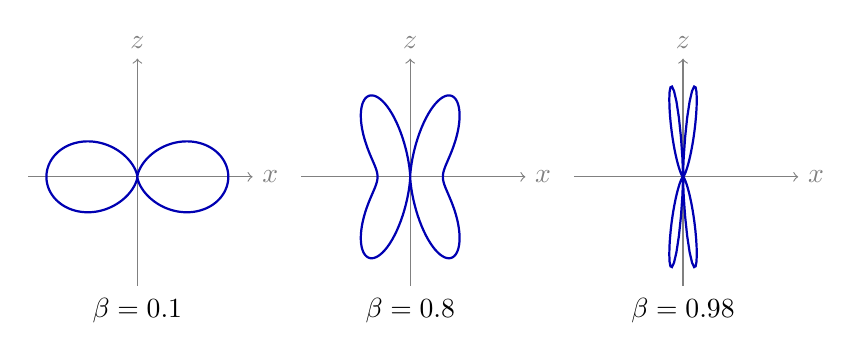
\begin{tikzpicture}[scale=.77]
\begin{scope}[xshift=0.0cm]
\draw[->,gray] (-1.8,0)--(1.9,0) node[right]{$x$};
\draw[->,gray] (0,-1.8)--(0,1.95) node[above]{$z$};
\draw[blue!70!black,thick] plot coordinates {(0.00000,0.00000) (0.00001,0.00047) (0.00007,0.00190) (0.00022,0.00426) (0.00053,0.00756) (0.00103,0.01178) (0.00178,0.01692) (0.00282,0.02295) (0.00420,0.02985) (0.00596,0.03761) (0.00815,0.04620) (0.01081,0.05559) (0.01398,0.06575) (0.01770,0.07665) (0.02200,0.08826) (0.02694,0.10053) (0.03253,0.11343) (0.03880,0.12692) (0.04580,0.14095) (0.05353,0.15548) (0.06204,0.17046) (0.07134,0.18585) (0.08145,0.20159) (0.09238,0.21763) (0.10415,0.23393) (0.11678,0.25043) (0.13026,0.26708) (0.14461,0.28382) (0.15983,0.30060) (0.17592,0.31736) (0.19287,0.33406) (0.21068,0.35062) (0.22934,0.36701) (0.24883,0.38317) (0.26916,0.39904) (0.29029,0.41457) (0.31220,0.42971) (0.33489,0.44441) (0.35831,0.45862) (0.38245,0.47228) (0.40726,0.48536) (0.43273,0.49780) (0.45882,0.50957) (0.48548,0.52062) (0.51269,0.53090) (0.54039,0.54039) (0.56855,0.54904) (0.59712,0.55683) (0.62606,0.56371) (0.65532,0.56966) (0.68485,0.57466) (0.71460,0.57867) (0.74451,0.58168) (0.77454,0.58366) (0.80464,0.58460) (0.83474,0.58449) (0.86480,0.58331) (0.89475,0.58106) (0.92455,0.57773) (0.95414,0.57331) (0.98347,0.56780) (1.01247,0.56122) (1.04109,0.55356) (1.06929,0.54483) (1.09699,0.53504) (1.12416,0.52421) (1.15074,0.51234) (1.17668,0.49947) (1.20192,0.48561) (1.22642,0.47078) (1.25013,0.45501) (1.27300,0.43833) (1.29499,0.42077) (1.31605,0.40236) (1.33615,0.38313) (1.35523,0.36313) (1.37327,0.34240) (1.39023,0.32096) (1.40608,0.29887) (1.42077,0.27617) (1.43429,0.25290) (1.44660,0.22912) (1.45769,0.20486) (1.46752,0.18019) (1.47609,0.15514) (1.48336,0.12978) (1.48934,0.10414) (1.49399,0.07830) (1.49733,0.05229) (1.49933,0.02617) (1.50000,0.00000) (1.49933,-0.02617) (1.49733,-0.05229) (1.49399,-0.07830) (1.48934,-0.10414) (1.48336,-0.12978) (1.47609,-0.15514) (1.46752,-0.18019) (1.45769,-0.20486) (1.44660,-0.22912) (1.43429,-0.25290) (1.42077,-0.27617) (1.40608,-0.29887) (1.39023,-0.32096) (1.37327,-0.34240) (1.35523,-0.36313) (1.33615,-0.38313) (1.31605,-0.40236) (1.29499,-0.42077) (1.27300,-0.43833) (1.25013,-0.45501) (1.22642,-0.47078) (1.20192,-0.48561) (1.17668,-0.49947) (1.15074,-0.51234) (1.12416,-0.52421) (1.09699,-0.53504) (1.06929,-0.54483) (1.04109,-0.55356) (1.01247,-0.56122) (0.98347,-0.56780) (0.95414,-0.57331) (0.92455,-0.57773) (0.89475,-0.58106) (0.86480,-0.58331) (0.83474,-0.58449) (0.80464,-0.58460) (0.77454,-0.58366) (0.74451,-0.58168) (0.71460,-0.57867) (0.68485,-0.57466) (0.65532,-0.56966) (0.62606,-0.56371) (0.59712,-0.55683) (0.56855,-0.54904) (0.54039,-0.54039) (0.51269,-0.53090) (0.48548,-0.52062) (0.45882,-0.50957) (0.43273,-0.49780) (0.40726,-0.48536) (0.38245,-0.47228) (0.35831,-0.45862) (0.33489,-0.44441) (0.31220,-0.42971) (0.29029,-0.41457) (0.26916,-0.39904) (0.24883,-0.38317) (0.22934,-0.36701) (0.21068,-0.35062) (0.19287,-0.33406) (0.17592,-0.31736) (0.15983,-0.30060) (0.14461,-0.28382) (0.13026,-0.26708) (0.11678,-0.25043) (0.10415,-0.23393) (0.09238,-0.21763) (0.08145,-0.20159) (0.07134,-0.18585) (0.06204,-0.17046) (0.05353,-0.15548) (0.04580,-0.14095) (0.03880,-0.12692) (0.03253,-0.11343) (0.02694,-0.10053) (0.02200,-0.08826) (0.01770,-0.07665) (0.01398,-0.06575) (0.01081,-0.05559) (0.00815,-0.04620) (0.00596,-0.03761) (0.00420,-0.02985) (0.00282,-0.02295) (0.00178,-0.01692) (0.00103,-0.01178) (0.00053,-0.00756) (0.00022,-0.00426) (0.00007,-0.00190) (0.00001,-0.00047) (0.00000,-0.00000) (-0.00001,-0.00047) (-0.00007,-0.00190) (-0.00022,-0.00426) (-0.00053,-0.00756) (-0.00103,-0.01178) (-0.00178,-0.01692) (-0.00282,-0.02295) (-0.00420,-0.02985) (-0.00596,-0.03761) (-0.00815,-0.04620) (-0.01081,-0.05559) (-0.01398,-0.06575) (-0.01770,-0.07665) (-0.02200,-0.08826) (-0.02694,-0.10053) (-0.03253,-0.11343) (-0.03880,-0.12692) (-0.04580,-0.14095) (-0.05353,-0.15548) (-0.06204,-0.17046) (-0.07134,-0.18585) (-0.08145,-0.20159) (-0.09238,-0.21763) (-0.10415,-0.23393) (-0.11678,-0.25043) (-0.13026,-0.26708) (-0.14461,-0.28382) (-0.15983,-0.30060) (-0.17592,-0.31736) (-0.19287,-0.33406) (-0.21068,-0.35062) (-0.22934,-0.36701) (-0.24883,-0.38317) (-0.26916,-0.39904) (-0.29029,-0.41457) (-0.31220,-0.42971) (-0.33489,-0.44441) (-0.35831,-0.45862) (-0.38245,-0.47228) (-0.40726,-0.48536) (-0.43273,-0.49780) (-0.45882,-0.50957) (-0.48548,-0.52062) (-0.51269,-0.53090) (-0.54039,-0.54039) (-0.56855,-0.54904) (-0.59712,-0.55683) (-0.62606,-0.56371) (-0.65532,-0.56966) (-0.68485,-0.57466) (-0.71460,-0.57867) (-0.74451,-0.58168) (-0.77454,-0.58366) (-0.80464,-0.58460) (-0.83474,-0.58449) (-0.86480,-0.58331) (-0.89475,-0.58106) (-0.92455,-0.57773) (-0.95414,-0.57331) (-0.98347,-0.56780) (-1.01247,-0.56122) (-1.04109,-0.55356) (-1.06929,-0.54483) (-1.09699,-0.53504) (-1.12416,-0.52421) (-1.15074,-0.51234) (-1.17668,-0.49947) (-1.20192,-0.48561) (-1.22642,-0.47078) (-1.25013,-0.45501) (-1.27300,-0.43833) (-1.29499,-0.42077) (-1.31605,-0.40236) (-1.33615,-0.38313) (-1.35523,-0.36313) (-1.37327,-0.34240) (-1.39023,-0.32096) (-1.40608,-0.29887) (-1.42077,-0.27617) (-1.43429,-0.25290) (-1.44660,-0.22912) (-1.45769,-0.20486) (-1.46752,-0.18019) (-1.47609,-0.15514) (-1.48336,-0.12978) (-1.48934,-0.10414) (-1.49399,-0.07830) (-1.49733,-0.05229) (-1.49933,-0.02617) (-1.50000,-0.00000) (-1.49933,0.02617) (-1.49733,0.05229) (-1.49399,0.07830) (-1.48934,0.10414) (-1.48336,0.12978) (-1.47609,0.15514) (-1.46752,0.18019) (-1.45769,0.20486) (-1.44660,0.22912) (-1.43429,0.25290) (-1.42077,0.27617) (-1.40608,0.29887) (-1.39023,0.32096) (-1.37327,0.34240) (-1.35523,0.36313) (-1.33615,0.38313) (-1.31605,0.40236) (-1.29499,0.42077) (-1.27300,0.43833) (-1.25013,0.45501) (-1.22642,0.47078) (-1.20192,0.48561) (-1.17668,0.49947) (-1.15074,0.51234) (-1.12416,0.52421) (-1.09699,0.53504) (-1.06929,0.54483) (-1.04109,0.55356) (-1.01247,0.56122) (-0.98347,0.56780) (-0.95414,0.57331) (-0.92455,0.57773) (-0.89475,0.58106) (-0.86480,0.58331) (-0.83474,0.58449) (-0.80464,0.58460) (-0.77454,0.58366) (-0.74451,0.58168) (-0.71460,0.57867) (-0.68485,0.57466) (-0.65532,0.56966) (-0.62606,0.56371) (-0.59712,0.55683) (-0.56855,0.54904) (-0.54039,0.54039) (-0.51269,0.53090) (-0.48548,0.52062) (-0.45882,0.50957) (-0.43273,0.49780) (-0.40726,0.48536) (-0.38245,0.47228) (-0.35831,0.45862) (-0.33489,0.44441) (-0.31220,0.42971) (-0.29029,0.41457) (-0.26916,0.39904) (-0.24883,0.38317) (-0.22934,0.36701) (-0.21068,0.35062) (-0.19287,0.33406) (-0.17592,0.31736) (-0.15983,0.30060) (-0.14461,0.28382) (-0.13026,0.26708) (-0.11678,0.25043) (-0.10415,0.23393) (-0.09238,0.21763) (-0.08145,0.20159) (-0.07134,0.18585) (-0.06204,0.17046) (-0.05353,0.15548) (-0.04580,0.14095) (-0.03880,0.12692) (-0.03253,0.11343) (-0.02694,0.10053) (-0.02200,0.08826) (-0.01770,0.07665) (-0.01398,0.06575) (-0.01081,0.05559) (-0.00815,0.04620) (-0.00596,0.03761) (-0.00420,0.02985) (-0.00282,0.02295) (-0.00178,0.01692) (-0.00103,0.01178) (-0.00053,0.00756) (-0.00022,0.00426) (-0.00007,0.00190) (-0.00001,0.00047) (-0.00000,0.00000)};
\node at (0,-2.2) {$\beta=0.1$};
\end{scope}
\begin{scope}[xshift=4.5cm]
\draw[->,gray] (-1.8,0)--(1.9,0) node[right]{$x$};
\draw[->,gray] (0,-1.8)--(0,1.95) node[above]{$z$};
\draw[blue!70!black,thick] plot coordinates {(0.00000,0.00000) (0.00012,0.00679) (0.00094,0.02697) (0.00315,0.06002) (0.00735,0.10509) (0.01409,0.16104) (0.02380,0.22647) (0.03681,0.29982) (0.05332,0.37938) (0.07339,0.46336) (0.09697,0.54997) (0.12391,0.63747) (0.15393,0.72419) (0.18669,0.80863) (0.22176,0.88942) (0.25868,0.96541) (0.29696,1.03561) (0.33608,1.09928) (0.37556,1.15585) (0.41490,1.20496) (0.45367,1.24644) (0.49144,1.28025) (0.52786,1.30651) (0.56262,1.32545) (0.59546,1.33742) (0.62617,1.34282) (0.65459,1.34211) (0.68063,1.33580) (0.70421,1.32442) (0.72531,1.30850) (0.74396,1.28857) (0.76018,1.26515) (0.77405,1.23874) (0.78566,1.20981) (0.79511,1.17880) (0.80252,1.14612) (0.80802,1.11215) (0.81175,1.07722) (0.81382,1.04165) (0.81440,1.00569) (0.81360,0.96961) (0.81156,0.93359) (0.80840,0.89782) (0.80426,0.86246) (0.79925,0.82764) (0.79347,0.79347) (0.78703,0.76002) (0.78003,0.72739) (0.77255,0.69561) (0.76469,0.66473) (0.75651,0.63479) (0.74809,0.60579) (0.73949,0.57775) (0.73076,0.55067) (0.72196,0.52454) (0.71314,0.49935) (0.70434,0.47508) (0.69559,0.45172) (0.68693,0.42924) (0.67840,0.40762) (0.67001,0.38683) (0.66179,0.36683) (0.65375,0.34761) (0.64593,0.32912) (0.63833,0.31133) (0.63097,0.29422) (0.62385,0.27776) (0.61699,0.26190) (0.61040,0.24662) (0.60408,0.23188) (0.59803,0.21767) (0.59227,0.20394) (0.58680,0.19066) (0.58162,0.17782) (0.57673,0.16537) (0.57213,0.15330) (0.56783,0.14158) (0.56383,0.13017) (0.56012,0.11906) (0.55671,0.10821) (0.55360,0.09761) (0.55079,0.08724) (0.54827,0.07705) (0.54605,0.06705) (0.54413,0.05719) (0.54250,0.04746) (0.54117,0.03784) (0.54013,0.02831) (0.53940,0.01884) (0.53895,0.00941) (0.53880,0.00000) (0.53895,-0.00941) (0.53940,-0.01884) (0.54013,-0.02831) (0.54117,-0.03784) (0.54250,-0.04746) (0.54413,-0.05719) (0.54605,-0.06705) (0.54827,-0.07705) (0.55079,-0.08724) (0.55360,-0.09761) (0.55671,-0.10821) (0.56012,-0.11906) (0.56383,-0.13017) (0.56783,-0.14158) (0.57213,-0.15330) (0.57673,-0.16537) (0.58162,-0.17782) (0.58680,-0.19066) (0.59227,-0.20394) (0.59803,-0.21767) (0.60408,-0.23188) (0.61040,-0.24662) (0.61699,-0.26190) (0.62385,-0.27776) (0.63097,-0.29422) (0.63833,-0.31133) (0.64593,-0.32912) (0.65375,-0.34761) (0.66179,-0.36683) (0.67001,-0.38683) (0.67840,-0.40762) (0.68693,-0.42924) (0.69559,-0.45172) (0.70434,-0.47508) (0.71314,-0.49935) (0.72196,-0.52454) (0.73076,-0.55067) (0.73949,-0.57775) (0.74809,-0.60579) (0.75651,-0.63479) (0.76469,-0.66473) (0.77255,-0.69561) (0.78003,-0.72739) (0.78703,-0.76002) (0.79347,-0.79347) (0.79925,-0.82764) (0.80426,-0.86246) (0.80840,-0.89782) (0.81156,-0.93359) (0.81360,-0.96961) (0.81440,-1.00569) (0.81382,-1.04165) (0.81175,-1.07722) (0.80802,-1.11215) (0.80252,-1.14612) (0.79511,-1.17880) (0.78566,-1.20981) (0.77405,-1.23874) (0.76018,-1.26515) (0.74396,-1.28857) (0.72531,-1.30850) (0.70421,-1.32442) (0.68063,-1.33580) (0.65459,-1.34211) (0.62617,-1.34282) (0.59546,-1.33742) (0.56262,-1.32545) (0.52786,-1.30651) (0.49144,-1.28025) (0.45367,-1.24644) (0.41490,-1.20496) (0.37556,-1.15585) (0.33608,-1.09928) (0.29696,-1.03561) (0.25868,-0.96541) (0.22176,-0.88942) (0.18669,-0.80863) (0.15393,-0.72419) (0.12391,-0.63747) (0.09697,-0.54997) (0.07339,-0.46336) (0.05332,-0.37938) (0.03681,-0.29982) (0.02380,-0.22647) (0.01409,-0.16104) (0.00735,-0.10509) (0.00315,-0.06002) (0.00094,-0.02697) (0.00012,-0.00679) (0.00000,-0.00000) (-0.00012,-0.00679) (-0.00094,-0.02697) (-0.00315,-0.06002) (-0.00735,-0.10509) (-0.01409,-0.16104) (-0.02380,-0.22647) (-0.03681,-0.29982) (-0.05332,-0.37938) (-0.07339,-0.46336) (-0.09697,-0.54997) (-0.12391,-0.63747) (-0.15393,-0.72419) (-0.18669,-0.80863) (-0.22176,-0.88942) (-0.25868,-0.96541) (-0.29696,-1.03561) (-0.33608,-1.09928) (-0.37556,-1.15585) (-0.41490,-1.20496) (-0.45367,-1.24644) (-0.49144,-1.28025) (-0.52786,-1.30651) (-0.56262,-1.32545) (-0.59546,-1.33742) (-0.62617,-1.34282) (-0.65459,-1.34211) (-0.68063,-1.33580) (-0.70421,-1.32442) (-0.72531,-1.30850) (-0.74396,-1.28857) (-0.76018,-1.26515) (-0.77405,-1.23874) (-0.78566,-1.20981) (-0.79511,-1.17880) (-0.80252,-1.14612) (-0.80802,-1.11215) (-0.81175,-1.07722) (-0.81382,-1.04165) (-0.81440,-1.00569) (-0.81360,-0.96961) (-0.81156,-0.93359) (-0.80840,-0.89782) (-0.80426,-0.86246) (-0.79925,-0.82764) (-0.79347,-0.79347) (-0.78703,-0.76002) (-0.78003,-0.72739) (-0.77255,-0.69561) (-0.76469,-0.66473) (-0.75651,-0.63479) (-0.74809,-0.60579) (-0.73949,-0.57775) (-0.73076,-0.55067) (-0.72196,-0.52454) (-0.71314,-0.49935) (-0.70434,-0.47508) (-0.69559,-0.45172) (-0.68693,-0.42924) (-0.67840,-0.40762) (-0.67001,-0.38683) (-0.66179,-0.36683) (-0.65375,-0.34761) (-0.64593,-0.32912) (-0.63833,-0.31133) (-0.63097,-0.29422) (-0.62385,-0.27776) (-0.61699,-0.26190) (-0.61040,-0.24662) (-0.60408,-0.23188) (-0.59803,-0.21767) (-0.59227,-0.20394) (-0.58680,-0.19066) (-0.58162,-0.17782) (-0.57673,-0.16537) (-0.57213,-0.15330) (-0.56783,-0.14158) (-0.56383,-0.13017) (-0.56012,-0.11906) (-0.55671,-0.10821) (-0.55360,-0.09761) (-0.55079,-0.08724) (-0.54827,-0.07705) (-0.54605,-0.06705) (-0.54413,-0.05719) (-0.54250,-0.04746) (-0.54117,-0.03784) (-0.54013,-0.02831) (-0.53940,-0.01884) (-0.53895,-0.00941) (-0.53880,-0.00000) (-0.53895,0.00941) (-0.53940,0.01884) (-0.54013,0.02831) (-0.54117,0.03784) (-0.54250,0.04746) (-0.54413,0.05719) (-0.54605,0.06705) (-0.54827,0.07705) (-0.55079,0.08724) (-0.55360,0.09761) (-0.55671,0.10821) (-0.56012,0.11906) (-0.56383,0.13017) (-0.56783,0.14158) (-0.57213,0.15330) (-0.57673,0.16537) (-0.58162,0.17782) (-0.58680,0.19066) (-0.59227,0.20394) (-0.59803,0.21767) (-0.60408,0.23188) (-0.61040,0.24662) (-0.61699,0.26190) (-0.62385,0.27776) (-0.63097,0.29422) (-0.63833,0.31133) (-0.64593,0.32912) (-0.65375,0.34761) (-0.66179,0.36683) (-0.67001,0.38683) (-0.67840,0.40762) (-0.68693,0.42924) (-0.69559,0.45172) (-0.70434,0.47508) (-0.71314,0.49935) (-0.72196,0.52454) (-0.73076,0.55067) (-0.73949,0.57775) (-0.74809,0.60579) (-0.75651,0.63479) (-0.76469,0.66473) (-0.77255,0.69561) (-0.78003,0.72739) (-0.78703,0.76002) (-0.79347,0.79347) (-0.79925,0.82764) (-0.80426,0.86246) (-0.80840,0.89782) (-0.81156,0.93359) (-0.81360,0.96961) (-0.81440,1.00569) (-0.81382,1.04165) (-0.81175,1.07722) (-0.80802,1.11215) (-0.80252,1.14612) (-0.79511,1.17880) (-0.78566,1.20981) (-0.77405,1.23874) (-0.76018,1.26515) (-0.74396,1.28857) (-0.72531,1.30850) (-0.70421,1.32442) (-0.68063,1.33580) (-0.65459,1.34211) (-0.62617,1.34282) (-0.59546,1.33742) (-0.56262,1.32545) (-0.52786,1.30651) (-0.49144,1.28025) (-0.45367,1.24644) (-0.41490,1.20496) (-0.37556,1.15585) (-0.33608,1.09928) (-0.29696,1.03561) (-0.25868,0.96541) (-0.22176,0.88942) (-0.18669,0.80863) (-0.15393,0.72419) (-0.12391,0.63747) (-0.09697,0.54997) (-0.07339,0.46336) (-0.05332,0.37938) (-0.03681,0.29982) (-0.02380,0.22647) (-0.01409,0.16104) (-0.00735,0.10509) (-0.00315,0.06002) (-0.00094,0.02697) (-0.00012,0.00679) (-0.00000,0.00000)};
\node at (0,-2.2) {$\beta=0.8$};
\end{scope}
\begin{scope}[xshift=9.0cm]
\draw[->,gray] (-1.8,0)--(1.9,0) node[right]{$x$};
\draw[->,gray] (0,-1.8)--(0,1.95) node[above]{$z$};
\draw[blue!70!black,thick] plot coordinates {(0.00000,0.00000) (0.00154,0.08823) (0.01141,0.32673) (0.03401,0.64890) (0.06823,0.97567) (0.10874,1.24292) (0.14881,1.41588) (0.18280,1.48882) (0.20742,1.47585) (0.22175,1.40008) (0.22663,1.28531) (0.22383,1.15152) (0.21539,1.01332) (0.20322,0.88023) (0.18891,0.75768) (0.17368,0.64819) (0.15839,0.55238) (0.14361,0.46973) (0.12969,0.39914) (0.11681,0.33924) (0.10505,0.28862) (0.09441,0.24596) (0.08486,0.21003) (0.07631,0.17977) (0.06869,0.15427) (0.06190,0.13275) (0.05587,0.11456) (0.05052,0.09915) (0.04576,0.08606) (0.04153,0.07491) (0.03776,0.06540) (0.03441,0.05726) (0.03142,0.05028) (0.02874,0.04426) (0.02636,0.03907) (0.02422,0.03458) (0.02229,0.03069) (0.02057,0.02730) (0.01901,0.02434) (0.01761,0.02175) (0.01635,0.01948) (0.01520,0.01749) (0.01416,0.01573) (0.01322,0.01418) (0.01237,0.01280) (0.01159,0.01159) (0.01087,0.01050) (0.01022,0.00953) (0.00963,0.00867) (0.00909,0.00790) (0.00859,0.00721) (0.00813,0.00658) (0.00771,0.00602) (0.00732,0.00552) (0.00697,0.00506) (0.00664,0.00465) (0.00633,0.00427) (0.00605,0.00393) (0.00579,0.00362) (0.00555,0.00334) (0.00533,0.00308) (0.00513,0.00284) (0.00494,0.00262) (0.00476,0.00243) (0.00460,0.00224) (0.00444,0.00207) (0.00430,0.00192) (0.00417,0.00177) (0.00405,0.00164) (0.00394,0.00151) (0.00384,0.00140) (0.00374,0.00129) (0.00365,0.00119) (0.00357,0.00109) (0.00349,0.00100) (0.00342,0.00092) (0.00336,0.00084) (0.00330,0.00076) (0.00325,0.00069) (0.00320,0.00062) (0.00316,0.00056) (0.00312,0.00049) (0.00309,0.00043) (0.00306,0.00038) (0.00303,0.00032) (0.00301,0.00026) (0.00299,0.00021) (0.00298,0.00016) (0.00297,0.00010) (0.00296,0.00005) (0.00296,0.00000) (0.00296,-0.00005) (0.00297,-0.00010) (0.00298,-0.00016) (0.00299,-0.00021) (0.00301,-0.00026) (0.00303,-0.00032) (0.00306,-0.00038) (0.00309,-0.00043) (0.00312,-0.00049) (0.00316,-0.00056) (0.00320,-0.00062) (0.00325,-0.00069) (0.00330,-0.00076) (0.00336,-0.00084) (0.00342,-0.00092) (0.00349,-0.00100) (0.00357,-0.00109) (0.00365,-0.00119) (0.00374,-0.00129) (0.00384,-0.00140) (0.00394,-0.00151) (0.00405,-0.00164) (0.00417,-0.00177) (0.00430,-0.00192) (0.00444,-0.00207) (0.00460,-0.00224) (0.00476,-0.00243) (0.00494,-0.00262) (0.00513,-0.00284) (0.00533,-0.00308) (0.00555,-0.00334) (0.00579,-0.00362) (0.00605,-0.00393) (0.00633,-0.00427) (0.00664,-0.00465) (0.00697,-0.00506) (0.00732,-0.00552) (0.00771,-0.00602) (0.00813,-0.00658) (0.00859,-0.00721) (0.00909,-0.00790) (0.00963,-0.00867) (0.01022,-0.00953) (0.01087,-0.01050) (0.01159,-0.01159) (0.01237,-0.01280) (0.01322,-0.01418) (0.01416,-0.01573) (0.01520,-0.01749) (0.01635,-0.01948) (0.01761,-0.02175) (0.01901,-0.02434) (0.02057,-0.02730) (0.02229,-0.03069) (0.02422,-0.03458) (0.02636,-0.03907) (0.02874,-0.04426) (0.03142,-0.05028) (0.03441,-0.05726) (0.03776,-0.06540) (0.04153,-0.07491) (0.04576,-0.08606) (0.05052,-0.09915) (0.05587,-0.11456) (0.06190,-0.13275) (0.06869,-0.15427) (0.07631,-0.17977) (0.08486,-0.21003) (0.09441,-0.24596) (0.10505,-0.28862) (0.11681,-0.33924) (0.12969,-0.39914) (0.14361,-0.46973) (0.15839,-0.55238) (0.17368,-0.64819) (0.18891,-0.75768) (0.20322,-0.88023) (0.21539,-1.01332) (0.22383,-1.15152) (0.22663,-1.28531) (0.22175,-1.40008) (0.20742,-1.47585) (0.18280,-1.48882) (0.14881,-1.41588) (0.10874,-1.24292) (0.06823,-0.97567) (0.03401,-0.64890) (0.01141,-0.32673) (0.00154,-0.08823) (0.00000,-0.00000) (-0.00154,-0.08823) (-0.01141,-0.32673) (-0.03401,-0.64890) (-0.06823,-0.97567) (-0.10874,-1.24292) (-0.14881,-1.41588) (-0.18280,-1.48882) (-0.20742,-1.47585) (-0.22175,-1.40008) (-0.22663,-1.28531) (-0.22383,-1.15152) (-0.21539,-1.01332) (-0.20322,-0.88023) (-0.18891,-0.75768) (-0.17368,-0.64819) (-0.15839,-0.55238) (-0.14361,-0.46973) (-0.12969,-0.39914) (-0.11681,-0.33924) (-0.10505,-0.28862) (-0.09441,-0.24596) (-0.08486,-0.21003) (-0.07631,-0.17977) (-0.06869,-0.15427) (-0.06190,-0.13275) (-0.05587,-0.11456) (-0.05052,-0.09915) (-0.04576,-0.08606) (-0.04153,-0.07491) (-0.03776,-0.06540) (-0.03441,-0.05726) (-0.03142,-0.05028) (-0.02874,-0.04426) (-0.02636,-0.03907) (-0.02422,-0.03458) (-0.02229,-0.03069) (-0.02057,-0.02730) (-0.01901,-0.02434) (-0.01761,-0.02175) (-0.01635,-0.01948) (-0.01520,-0.01749) (-0.01416,-0.01573) (-0.01322,-0.01418) (-0.01237,-0.01280) (-0.01159,-0.01159) (-0.01087,-0.01050) (-0.01022,-0.00953) (-0.00963,-0.00867) (-0.00909,-0.00790) (-0.00859,-0.00721) (-0.00813,-0.00658) (-0.00771,-0.00602) (-0.00732,-0.00552) (-0.00697,-0.00506) (-0.00664,-0.00465) (-0.00633,-0.00427) (-0.00605,-0.00393) (-0.00579,-0.00362) (-0.00555,-0.00334) (-0.00533,-0.00308) (-0.00513,-0.00284) (-0.00494,-0.00262) (-0.00476,-0.00243) (-0.00460,-0.00224) (-0.00444,-0.00207) (-0.00430,-0.00192) (-0.00417,-0.00177) (-0.00405,-0.00164) (-0.00394,-0.00151) (-0.00384,-0.00140) (-0.00374,-0.00129) (-0.00365,-0.00119) (-0.00357,-0.00109) (-0.00349,-0.00100) (-0.00342,-0.00092) (-0.00336,-0.00084) (-0.00330,-0.00076) (-0.00325,-0.00069) (-0.00320,-0.00062) (-0.00316,-0.00056) (-0.00312,-0.00049) (-0.00309,-0.00043) (-0.00306,-0.00038) (-0.00303,-0.00032) (-0.00301,-0.00026) (-0.00299,-0.00021) (-0.00298,-0.00016) (-0.00297,-0.00010) (-0.00296,-0.00005) (-0.00296,-0.00000) (-0.00296,0.00005) (-0.00297,0.00010) (-0.00298,0.00016) (-0.00299,0.00021) (-0.00301,0.00026) (-0.00303,0.00032) (-0.00306,0.00038) (-0.00309,0.00043) (-0.00312,0.00049) (-0.00316,0.00056) (-0.00320,0.00062) (-0.00325,0.00069) (-0.00330,0.00076) (-0.00336,0.00084) (-0.00342,0.00092) (-0.00349,0.00100) (-0.00357,0.00109) (-0.00365,0.00119) (-0.00374,0.00129) (-0.00384,0.00140) (-0.00394,0.00151) (-0.00405,0.00164) (-0.00417,0.00177) (-0.00430,0.00192) (-0.00444,0.00207) (-0.00460,0.00224) (-0.00476,0.00243) (-0.00494,0.00262) (-0.00513,0.00284) (-0.00533,0.00308) (-0.00555,0.00334) (-0.00579,0.00362) (-0.00605,0.00393) (-0.00633,0.00427) (-0.00664,0.00465) (-0.00697,0.00506) (-0.00732,0.00552) (-0.00771,0.00602) (-0.00813,0.00658) (-0.00859,0.00721) (-0.00909,0.00790) (-0.00963,0.00867) (-0.01022,0.00953) (-0.01087,0.01050) (-0.01159,0.01159) (-0.01237,0.01280) (-0.01322,0.01418) (-0.01416,0.01573) (-0.01520,0.01749) (-0.01635,0.01948) (-0.01761,0.02175) (-0.01901,0.02434) (-0.02057,0.02730) (-0.02229,0.03069) (-0.02422,0.03458) (-0.02636,0.03907) (-0.02874,0.04426) (-0.03142,0.05028) (-0.03441,0.05726) (-0.03776,0.06540) (-0.04153,0.07491) (-0.04576,0.08606) (-0.05052,0.09915) (-0.05587,0.11456) (-0.06190,0.13275) (-0.06869,0.15427) (-0.07631,0.17977) (-0.08486,0.21003) (-0.09441,0.24596) (-0.10505,0.28862) (-0.11681,0.33924) (-0.12969,0.39914) (-0.14361,0.46973) (-0.15839,0.55238) (-0.17368,0.64819) (-0.18891,0.75768) (-0.20322,0.88023) (-0.21539,1.01332) (-0.22383,1.15152) (-0.22663,1.28531) (-0.22175,1.40008) (-0.20742,1.47585) (-0.18280,1.48882) (-0.14881,1.41588) (-0.10874,1.24292) (-0.06823,0.97567) (-0.03401,0.64890) (-0.01141,0.32673) (-0.00154,0.08823) (-0.00000,0.00000)};
\node at (0,-2.2) {$\beta=0.98$};
\end{scope}
\end{tikzpicture}
\end{center}

\Needspace{5\baselineskip}
\par\bigskip
\noindent\textbf{14.13}\quad Show explicitly by use of the Poisson sum formula or other means that, if the motion of a radiating particle repeats itself with periodicity $T$, the continuous frequency spectrum becomes a discrete spectrum containing frequencies that are integral multiples of the fundamental. Show that a general expression for the time-averaged power radiated per unit solid angle in each multiple $m$ of the fundamental frequency $\omega_{0}=2\pi/T$ is:
\[
\frac{dP_{m}}{d\Omega}=\frac{e^{2}\omega_{0}^{4}m^{2}}{(2\pi c)^{3}}\left|\int_{0}^{2\pi/\omega_{0}}\mathbf{v}(t)\times\mathbf{n}\,\exp\!\left[im\omega_{0}\!\left(t-\frac{\mathbf{n}\cdot\mathbf{x}(t)}{c}\right)\right]dt\right|^{2}
\]
\solution

Let $\omega>0$ and write the one-period vector integral
\[
\mathbf F_T(\omega)=\int_0^T\mathbf v(t)\times\mathbf n
\exp\{i\omega[t-\mathbf n\cdot\mathbf x(t)/c]\}\,dt.
\]
For $M$ repeated periods, periodicity of both $\mathbf x$ and $\mathbf v$
makes the full transform
$\mathbf F_T(\omega)\sum_{j=0}^{M-1}e^{ij\omega T}$.
The spectral energy formula is
$e^2\omega^2|\mathbf F|^2/(4\pi^2c^3)$.
Divide it by the observation duration $MT$ and use the distributional
limit of the squared geometric sum:
\[
\frac1{MT}\left|\sum_{j=0}^{M-1}e^{ij\omega T}\right|^2
\longrightarrow\frac{2\pi}{T^2}
\sum_{m=-\infty}^{\infty}\delta(\omega-m\omega_0).
\]
To check the normalization, expand the square as
$\sum_{s=-(M-1)}^{M-1}(M-|s|)e^{is\omega T}$.
After division by $MT$, its limit is
$T^{-1}\sum_s e^{is\omega T}$; Poisson summation gives
$\sum_s e^{is\omega T}=(2\pi/T)\sum_m\delta(\omega-2\pi m/T)$.
Thus the weight of the positive line $\omega=m\omega_0$ is
\[
\boxed{\frac{dP_m}{d\Omega}
=\frac{e^2(m\omega_0)^2}{2\pi c^3T^2}
|\mathbf F_T(m\omega_0)|^2
=\frac{e^2\omega_0^4m^2}{(2\pi c)^3}
|\mathbf F_T(m\omega_0)|^2.}
\]
The $m=0$ line does not radiate because of the explicit frequency square.
Finite $M$ replaces each delta by a narrow peak of width of order
$1/(MT)$; the infinite-time limit is taken after dividing by duration,
so no undefined square of a delta function is used.

\Needspace{5\baselineskip}
\par\bigskip
\noindent\textbf{14.14}\quad\begin{enumerate}
\item[(a)] Show that for the simple harmonic motion of a charge discussed in Problem 14.12 the average power radiated per unit solid angle in the $m$th harmonic is
\[
\frac{dP_{m}}{d\Omega}=\frac{e^{2}c\beta^{2}}{2\pi a^{2}}\,m^{2}\tan^{2}\theta\,J_{m}^{2}(m\beta\cos\theta)
\]
\item[(b)] Show that in the nonrelativistic limit the total power radiated is all in the fundamental and has the value
\[
P\simeq\frac{2}{3}\frac{e^{2}}{c^{3}}\,\omega_{0}^{4}\,\overline{a^{2}}
\]
where $\overline{a^{2}}$ is the mean square amplitude of oscillation.
\end{enumerate}
\solution

\textbf{(a)} Set $u=\omega_0t$ and $b=\beta\cos\theta$ in 14.13.
The phase is $m(u-b\cos u)$ and $v_zdt=-a\sin u\,du$.
The needed Bessel representation is
\[
I_m(b)=\int_0^{2\pi}e^{im(u-b\cos u)}du
=2\pi(-i)^mJ_m(mb).
\]
Integrating the derivative of the exponential over its full period gives
\[
0=im\int_0^{2\pi}(1+b\sin u)e^{im(u-b\cos u)}du.
\]
Thus $\int\sin u\,e^{im(u-b\cos u)}du=-I_m/b$, and the magnitude of
the transverse velocity integral is
$2\pi a|\tan\theta\,J_m(m\beta\cos\theta)|/\beta$.
Its squared magnitude in 14.13 gives
\[
\boxed{\frac{dP_m}{d\Omega}
=\frac{e^2c\beta^2}{2\pi a^2}
 m^2\tan^2\theta J_m(m\beta\cos\theta)^2.}
\]
The apparent singularity at $\cos\theta=0$ is removable. There the
fundamental has a finite limit because $J_1(x)\sim x/2$, and every
$m>1$ term vanishes because $J_m(x)=O(x^m)$.

\textbf{(b)} For fixed $m$ and small $\beta$,
$J_m(m\beta\cos\theta)\simeq
(m\beta\cos\theta/2)^m/m!$. The $m$th power is thus of order
$\beta^{2m+2}$ in the displayed normalization; the fundamental dominates.
For $m=1$,
\[
\frac{dP_1}{d\Omega}\simeq
\frac{e^2c\beta^4}{8\pi a^2}\sin^2\theta,
\quad
P_1\simeq\frac{e^2c\beta^4}{3a^2}
=\frac{e^2\omega_0^4a^2}{3c^3}.
\]
With $\overline{z^2}=a^2/2$, the last expression is
$(2e^2/3c^3)\omega_0^4\overline{z^2}$, the stated formula with its
mean-square-amplitude notation $\overline{a^2}$.

\Needspace{5\baselineskip}
\par\bigskip
\noindent\textbf{14.15}\quad A particle of charge $e$ moves in a circular path of radius $R$ in the $x$-$y$ plane with a constant angular velocity $\omega_{0}$.
\begin{enumerate}
\item[(a)] Show that the exact expression for the angular distribution of power radiated into the $m$th multiple of $\omega_{0}$ is
\[
\frac{dP_{m}}{d\Omega}=\frac{e^{2}\omega_{0}^{4}R^{2}}{2\pi c^{3}}\,m^{2}\!\left\{\left[\frac{dJ_{m}(m\beta\sin\theta)}{d(m\beta\sin\theta)}\right]^{2}+\frac{\cot^{2}\theta}{\beta^{2}}\,J_{m}^{2}(m\beta\sin\theta)\right\}
\]
where $\beta=\omega_{0}R/c$, and $J_{m}(x)$ is the Bessel function of order $m$.
\item[(b)] Assume nonrelativistic motion and obtain an approximate result for $dP_{m}/d\Omega$. Show that the results of Problem 14.4b are obtained in this limit.
\item[(c)] Assume extreme relativistic motion and obtain the results found in the text for a relativistic particle in instantaneously circular motion. [\emph{Watson} (pp.~79, 249) may be of assistance to you.]
\end{enumerate}
\solution

\textbf{(a)} By axial symmetry take the observation azimuth to be zero,
$\mathbf n=(\sin\theta,0,\cos\theta)$, with transverse basis
$\boldsymbol\epsilon_\theta=(\cos\theta,0,-\sin\theta)$ and
$\boldsymbol\epsilon_\phi=(0,1,0)$. Put $u=\omega_0t$ and
$b=\beta\sin\theta$. The position and velocity integrals are
\[
\mathbf r=R(\cos u,\sin u,0),\qquad
\mathbf vdt=R(-\sin u,\cos u,0)du,
\]
with phase $m(u-b\cos u)$.
From 14.14, $\int\sin u\,e^{i\mathrm{phase}}du=-I_m/b$.
Differentiating $I_m(b)$ also gives
$\int\cos u\,e^{i\mathrm{phase}}du=(i/m)I'_m(b)
=2\pi i(-i)^mJ'_m(mb)$. Therefore the two transverse components of
the velocity integral are
\[
V_\theta=2\pi R(-i)^m\frac{\cot\theta}{\beta}J_m(mb),\qquad
V_\phi=2\pi iR(-i)^mJ'_m(mb).
\]
Their orthogonality makes the squared modulus a sum. Substitution in
14.13 yields the expression in the question, including its relative
$\beta^{-2}$ factor.

\textbf{(b)} For small $\beta$,
$J_m(x)\simeq(x/2)^m/m!$ and $J'_m(x)\simeq mJ_m(x)/x$.
At $x=m\beta\sin\theta$ this gives
\[
\boxed{\frac{dP_m}{d\Omega}\simeq
\frac{e^2\omega_0^2}{2\pi c}
\frac{m^{2m+2}\beta^{2m}}{2^{2m}(m!)^2}
\sin^{2m-2}\theta(1+\cos^2\theta).}
\]
Only $m=1$ survives to leading order; it equals
$e^2R^2\omega_0^4(1+\cos^2\theta)/(8\pi c^3)$, and its angular integral
is $2e^2R^2\omega_0^4/(3c^3)$, exactly 14.4(b).

\textbf{(c)} Write $\psi=\theta-\pi/2$ and
$A=\gamma^{-2}+\psi^2$. For $\gamma\gg1$, $|\psi|\ll1$,
$\beta\sin\theta=1-A/2+\cdots$.
Use $J_m(x)=\pi^{-1}\int_0^\pi\cos(mu-x\sin u)du$ for integer $m$.
In the large-$m$ region contributing to radiation, the phase near zero is
\[
mu-m\beta\sin\theta\sin u
\simeq\frac m2(Au+u^3/3).
\]
Put $u=\sqrt A\,s$ and $\xi=mA^{3/2}/3$. The Airy-integral identities
\[
\int_0^\infty\cos\left[\frac{3\xi}{2}(s+s^3/3)\right]ds
=\frac1{\sqrt3}K_{1/3}(\xi),\quad
\int_0^\infty s\sin\left[\frac{3\xi}{2}(s+s^3/3)\right]ds
=\frac1{\sqrt3}K_{2/3}(\xi)
\]
then give
\[
J_m(m\beta\sin\theta)\simeq\frac{\sqrt A}{\pi\sqrt3}K_{1/3}(\xi),
\quad
J'_m(m\beta\sin\theta)\simeq\frac A{\pi\sqrt3}K_{2/3}(\xi).
\]
The second relation follows by differentiating the integral with respect
to its argument before making the same small-$u$ expansion.
Part (a) consequently becomes
\[
\frac{dP_m}{d\Omega}\simeq
\frac{e^2\omega_0^2m^2}{6\pi^3c}A^2
\left[K_{2/3}^2(\xi)+\frac{\psi^2}{A}K_{1/3}^2(\xi)\right].
\]
For many closely spaced harmonics, divide by the spacing $\omega_0$
to get power per unit frequency. Multiplication by the orbit period
$2\pi/\omega_0$ converts this to the single-pulse energy spectrum:
\[
\boxed{\frac{d^2I}{d\omega d\Omega}\simeq
\frac{e^2}{3\pi^2c}\left(\frac{\omega\rho}{c}\right)^2A^2
\left[K_{2/3}^2(\xi)+\frac{\psi^2}{A}K_{1/3}^2(\xi)\right],}
\]
where $\rho=R\simeq c/\omega_0$,
$\omega_c=3\gamma^3c/(2\rho)$, and
$\xi=(\omega/2\omega_c)(1+\gamma^2\psi^2)^{3/2}$.
This is the instantaneously circular result (14.79), with its two
orthogonal polarization contributions retained.

\Needspace{5\baselineskip}
\par\bigskip
\noindent\textbf{14.16}\quad Exploiting the fact that $k_{0}d^{3}N/d^{3}k$, the number of quanta per invariant phase-space element $d^{3}k/k_{0}$, is a Lorentz-invariant quantity, show that the energy radiated per unit frequency interval per unit solid angle, (14.79), can be written in the invariant and coordinate-free form
\[
\hbar\omega\,\frac{d^{3}N}{d^{3}k}=\frac{4e^{2}}{3\pi^{2}m^{2}}\left[\frac{(p\cdot k)^{2}}{[d^{2}(p\cdot k)/d\tau^{2}]^{2}}\left(\frac{d(\boldsymbol{\epsilon}_{1}\cdot p)}{d\tau}\right)^{2}\!K_{2/3}^{2}(\xi)+\frac{(p\cdot k)(\boldsymbol{\epsilon}_{2}\cdot p)^{2}}{2[d^{2}(p\cdot k)/d\tau^{2}]}\,K_{1/3}^{2}(\xi)\right]
\]
where \erratum{the same ultrarelativistic local-curvature approximation as in (14.79) is understood,} $d\tau$ is the proper time interval of the particle of mass $m$, $p^{\mu}$ is the 4-momentum of the particle, $k^{\mu}$ is the 4-wave vector of the radiation, and $\boldsymbol{\epsilon}_{1}$, $\boldsymbol{\epsilon}_{2}$ are polarization vectors parallel to the acceleration and in the direction $\boldsymbol{\epsilon}_{1}\times\mathbf{k}$, respectively. The parameter is
\[
\xi=\frac{2\sqrt{2}}{3m}\cdot\frac{(p\cdot k)^{3/2}}{\left(|d^{2}(p\cdot k)/d\tau^{2}|\right)^{1/2}}
\]
This expression can be used to obtain the results of Problem 14.17 in an alternative manner. \emph{Hint}: In proceeding with a solution, it is useful to expand $\mathbf{k}\cdot\mathbf{r}(t)$ around $t=0$ in terms of the velocity, acceleration, etc.\ and compare with (14.72). One finds, for example, that $\omega c^{2}/\rho^{2}=-\mathbf{k}\cdot d^{2}\mathbf{v}(0)/dt^{2}$, and, because the energy is constant,
\[
\rho^{2}=\frac{\omega E^{3}}{m^{2}c^{4}\,|d^{2}(p\cdot k)/d\tau^{2}|}
\]
\solution

The result has the same local-curvature and ultrarelativistic accuracy
as (14.79); it is not an exact formula for arbitrary motion. Use metric
$(+,-,-,-)$. At the emission point choose fixed polarization four-vectors
$\epsilon_i^\mu=(0,\boldsymbol\epsilon_i)$ in the frame used for the
local circular calculation, and transform those four-vectors along with
$p$ and $k$ when changing frames.

Since $d^3k=(\omega^2/c^3)d\omega d\Omega$,
\[
\hbar\omega\frac{d^3N}{d^3k}
=\frac{c^3}{\omega^2}\frac{d^2I}{d\omega d\Omega}.
\]
The left side is invariant because the number of quanta and
$d^3k/k^0$ are invariant and $k^0=\omega/c$.
Let $A=\gamma^{-2}+\psi^2$, $E=\gamma mc^2$,
$Q=p\cdot k$, and $D=d^2(p\cdot k)/d\tau^2$.
In the local circular frame, the following reductions keep the same
leading terms as the spectral formula:
\[
Q=\frac{E\omega}{c^2}(1-\beta\cos\psi)
\simeq\frac{E\omega}{2c^2}A,
\qquad
\epsilon_2\cdot p\simeq\frac E c\psi
\quad\hbox{up to its unimportant sign}.
\]
For constant energy, $d/d\tau=\gamma d/dt$ and
$\mathbf p=\gamma m\mathbf v$. Expanding the phase gives
\[
\omega\left(t-\frac{\mathbf n\cdot\mathbf r(t)}c\right)
=\omega(1-\mathbf n\cdot\boldsymbol\beta)t
-\frac{\omega}{2c}\mathbf n\cdot\mathbf a\,t^2
-\frac{\omega}{6c}\mathbf n\cdot\dot{\mathbf a}\,t^3+\cdots.
\]
At closest alignment $\mathbf n\cdot\mathbf a=0$ and
$-\mathbf k\cdot\dot{\mathbf a}\simeq\omega c^2/\rho^2$.
Consequently
\[
D=-\gamma^3m\mathbf k\cdot\dot{\mathbf a}
\simeq\frac{\omega E^3}{m^2c^4\rho^2}>0,
\qquad
\left(\frac{d(\epsilon_1\cdot p)}{d\tau}\right)^2
\simeq\left(\gamma^2m\frac{c^2}{\rho}\right)^2
=\frac{E^4}{m^2c^4\rho^2}.
\]
These establish the hint's expression for $\rho^2$.
Substitution in the two proposed invariant coefficients gives, separately,
\[
\frac4{m^2}\frac{Q^2}{D^2}
\left(\frac{d(\epsilon_1\cdot p)}{d\tau}\right)^2
=\rho^2A^2,
\qquad
\frac4{m^2}\frac{Q(\epsilon_2\cdot p)^2}{2D}
=\rho^2A\psi^2.
\]
Also
\[
\frac{2\sqrt2}{3m}\frac{Q^{3/2}}{\sqrt{|D|}}
=\frac{\omega\rho}{3c}A^{3/2}=\xi.
\]
Multiplying (14.79) by $c^3/\omega^2$ now gives exactly the expression
in the question. Every factor $Q,D,\epsilon_i\cdot p$ and its proper-time
derivative is a Lorentz scalar under the stated simultaneous
transformation, so equality established in this convenient frame holds
in every frame, to the same approximation order.

\Needspace{5\baselineskip}
\par\bigskip
\noindent\textbf{14.17}\quad A particle of charge $e$ and mass $m$ moves relativistically in a helical path in a uniform magnetic field $\mathbf{B}$. The pitch angle of the helix is $\alpha$ ($\alpha=0$ corresponds to circular motion).
\begin{enumerate}
\item[(a)] By arguments similar to those of Section 14.4, show that an observer far from the helix \erratum{within the beaming cone, for $\gamma\gg1$ and $\gamma\cos\alpha\gg1$,} would detect radiation with a fundamental frequency
\[
\omega_{0}=\frac{\omega_{B}}{\cos^{2}\alpha}
\]
and that the spectrum would extend up to frequencies in the order of
\[
\omega_{c}=\frac{3}{2}\,\gamma^{3}\omega_{B}\cos\alpha
\]
where $\omega_{B}=eB/\gamma mc$. (Take care in determining the radius of curvature $\rho$ of the helical path.)
\item[(b)] From part a and the results of Section 14.6, show that the \emph{power} received by the observer per unit solid angle and per unit circular frequency interval is
\[
\frac{d^{2}P}{d\omega\;d\Omega}\simeq\frac{3e^{2}\gamma^{2}}{8\pi^{3}c}\frac{\omega_{B}}{\cos^{2}\alpha}\left(\frac{\omega}{\omega_{c}}\right)^{2}\!(1+\gamma^{2}\psi^{2})^{2}\!\left[K_{2/3}^{2}(\xi)+\frac{\gamma^{2}\psi^{2}}{1+\gamma^{2}\psi^{2}}\,K_{1/3}^{2}(\xi)\right]
\]
where $\omega_{B}$ and $\omega_{c}$ are defined above, $\xi=(\omega/2\omega_{c})(1+\gamma^{2}\psi^{2})^{3/2}$, and $\psi$ is the angle of observation measured relative to the particle's velocity vector, as in Fig.~14.9.
\end{enumerate}
\solution

Let the magnetic field define the $z$ axis. Then
$v_\perp=v\cos\alpha$, $v_\parallel=v\sin\alpha$, and the rotation
period in source time is $T=2\pi/\omega_B$.

\textbf{(a)} During one turn the particle advances
$\Delta z=v\sin\alpha T$. For an observer at polar angle $\theta$,
subtracting the path-length change from the source period gives the
exact far-observer period and its corresponding fundamental:
\[
T_{\rm obs}=T(1-\beta\sin\alpha\cos\theta),\qquad
\boxed{\omega_{\rm obs}=
\frac{\omega_B}{1-\beta\sin\alpha\cos\theta}.}
\]
The strong radiation is seen near
$\theta_0=\pi/2-\alpha$, where the velocity points toward the observer.
For $\gamma\gg1$ and $\gamma\cos\alpha\gg1$, its denominator is
$\cos^2\alpha$ to leading order; thus
$\omega_0\simeq\omega_B/\cos^2\alpha$ as stated.
The viewing and pitch qualifications are necessary: a general viewing
direction has the Doppler factor displayed above.

The helix's cylindrical radius is $r_L=v\cos\alpha/\omega_B$,
but its acceleration magnitude is $a=v\omega_B\cos\alpha$.
Since speed is constant, the curvature radius is
\[
\rho=\frac{v^2}{a}=\frac v{\omega_B\cos\alpha}
=\frac{r_L}{\cos^2\alpha},
\]
not $r_L$. The synchrotron cutoff scale is therefore
\[
\boxed{\omega_c=\frac{3\gamma^3c}{2\rho}
\simeq\frac32\gamma^3\omega_B\cos\alpha.}
\]

\textbf{(b)} In terms of $x=\omega/\omega_c$, the single-pulse spectrum
in 14.15 is
\[
\frac{d^2I}{d\omega d\Omega}
=\frac{3e^2\gamma^2}{4\pi^2c}x^2(1+\gamma^2\psi^2)^2
\left[K_{2/3}^2(\xi)+\frac{\gamma^2\psi^2}{1+\gamma^2\psi^2}
K_{1/3}^2(\xi)\right].
\]
This follows directly by replacing
$(\omega\rho/c)^2(\gamma^{-2}+\psi^2)^2$
by $(9/4)\gamma^2x^2(1+\gamma^2\psi^2)^2$.
The received mean power is the pulse energy divided by
$T_{\rm obs}\simeq2\pi\cos^2\alpha/\omega_B$; this produces the
coefficient $3e^2\gamma^2\omega_B/(8\pi^3c\cos^2\alpha)$ and exactly
the expression requested in part (b).
Here $\psi$ is the small displacement from closest alignment, as in the
local circular radiation formula. The approximation presumes that the
beaming cone does not collapse onto the field axis.

\Needspace{5\baselineskip}
\par\bigskip
\noindent\textbf{14.18}\quad\begin{enumerate}
\item[(a)] By comparison of (14.91) with (14.79), show that the frequency spectrum of the received power for the situation in Problem 14.17 is
\[
\frac{dP}{d\omega}=\left(\frac{\sqrt{3}e^{2}\gamma\omega_{B}}{2\pi c\,\cos\alpha}\right)\!G\!\left(\frac{\omega}{\omega_{c}}\right)
\]
where $G(x)=x\displaystyle\int_{x}^{\infty}K_{5/3}(t)\;dt$ and the other symbols are as in Problem 14.17. This expression shows that the \emph{shape} of the power spectrum in units of $\omega/\omega_{c}$ is unchanged by the spiraling.
\item[(b)] Show that the integral over frequencies yields
\[
P=\frac{2e^{2}\omega_{B}^{2}\gamma^{4}}{3c}
\]
Comparison with (14.31) shows that the total received power is independent of the pitch angle of motion.
\end{enumerate}
[In doing the integration over solid angles in part a, note that $\psi=0$ corresponds to $\theta=\pi/2-\alpha$.]
\solution

\textbf{(a)} For the circular orbit with the same curvature $\rho$,
write $\omega_{\rho}=c/\rho=\omega_B\cos\alpha$ to leading order.
Its spectral power, from (14.91), is
$\sqrt3e^2\gamma\omega_{\rho}G(\omega/\omega_c)/(2\pi c)$.
The helix has the same local pulse spectrum, but its received repetition
rate is $\omega_B/\cos^2\alpha$ rather than $\omega_{\rho}$: this
multiplies the angle-resolved power by $\cos^{-3}\alpha$.
The angular integration has a compensating geometric factor, because
\[
d\Omega\simeq2\pi\sin\theta_0\,d\psi
=2\pi\cos\alpha\,d\psi
\]
instead of $2\pi d\psi$ for the circular orbit. Combining these factors
with $\omega_{\rho}=\omega_B\cos\alpha$ gives
\[
\boxed{\frac{dP_{\rm rec}}{d\omega}
=\frac{\sqrt3e^2\gamma\omega_B}{2\pi c\cos\alpha}
G\left(\frac\omega{\omega_c}\right),\quad
G(x)=x\int_x^\infty K_{5/3}(t)dt.}
\]

\textbf{(b)} Interchange the positive integrals:
\[
\int_0^\infty G(x)dx
=\int_0^\infty K_{5/3}(t)\left(\int_0^t x\,dx\right)dt
=\frac12\int_0^\infty t^2K_{5/3}(t)dt.
\]
The Bessel integral
$\int_0^\infty t^{s-1}K_\nu(t)dt
=2^{s-2}\Gamma[(s+\nu)/2]\Gamma[(s-\nu)/2]$
with $s=3$ gives
\[
\int_0^\infty G(x)dx
=\Gamma(7/3)\Gamma(2/3)
=\frac49\Gamma(1/3)\Gamma(2/3)
=\frac{8\pi}{9\sqrt3}.
\]
Multiplication by the coefficient in (a) and
$\omega_c=3\gamma^3\omega_B\cos\alpha/2$ gives
\[
\boxed{P_{\rm rec}=\frac{2e^2\omega_B^2\gamma^4}{3c}.}
\]
This is the stated \emph{received} power in the beaming approximation.
The emitted energy per unit source time is instead
$P_{\rm emit}=2e^2\omega_B^2\gamma^4\beta^2\cos^2\alpha/(3c)$,
from the Li\'enard formula. The leading ratio
$P_{\rm rec}/P_{\rm emit}\simeq\cos^{-2}\alpha$ is the shortening of
the arrival interval, not extra energy generation. The small-$\cos\alpha$
limit must respect the qualifications of 14.17.

\Needspace{5\baselineskip}
\par\bigskip
\noindent\textbf{14.19}\quad Consider the angular and frequency spectrum of radiation produced by a magnetic moment in nonrelativistic motion, using (14.70) and the fact that a magnetization density $\mathcal{M}$ produces an effective current density $\mathbf{J}_{\mathrm{eff}}=c\nabla\times\mathcal{M}$.
\begin{enumerate}
\item[(a)] Show that a magnetic moment $\boldsymbol{\mu}$ with magnetization, $\mathcal{M}=\boldsymbol{\mu}(t)\,\delta[\mathbf{x}-\mathbf{r}(t)]$, in nonrelativistic motion gives a radiation intensity (energy radiated per unit solid angle per unit frequency interval),
\[
\frac{d^{2}I_{\mathrm{mag}}}{d\omega\;d\Omega}=\frac{\omega^{4}}{4\pi^{2}c^{3}}\left|\int dt\;\mathbf{n}\times\boldsymbol{\mu}(t)e^{i\omega(t-\mathbf{n}\cdot\mathbf{r}(t)/c)}\right|^{2}
\]
\item[(b)] The magnetic moment is located at the origin and is caused to precess by an external torque such that $\mu_{x}=\mu_{0}\sin\omega_{0}t$ and $\mu_{z}=\mu_{0}\cos\omega_{0}t$ for the time interval $t=-T/2$ to $t=T/2$, where $\omega_{0}T/2\pi\gg1$, \erratum{with smooth switching outside the long periodic interval}. Show that the frequency distribution of the radiation is very strongly peaked at $\omega=\omega_{0}$, that the angular distribution of radiation is proportional to $(1+\sin^{2}\theta\sin^{2}\phi)$, and that for $T\to\infty$, the total time-averaged power radiated is
\[
\langle P\rangle=\frac{2\omega_{0}^{4}}{3c^{3}}\,\mu_{0}^{2}
\]
Compare the result with the power calculated by the method of Section 9.3.
\end{enumerate}
\solution

\textbf{(a)} The Gaussian current spectral formula is
\[
\frac{d^2I}{d\omega d\Omega}
=\frac{\omega^2}{4\pi^2c^3}
\left|\int dt\,d^3x\;\mathbf n\times\mathbf J(\mathbf x,t)
 e^{i\omega(t-\mathbf n\cdot\mathbf x/c)}\right|^2.
\]
For $\mathbf J=c\nabla\times\boldsymbol{\mathcal M}$, integration by
parts puts the curl on the spatial exponential and gives
\[
\int\mathbf J e^{-i(\omega/c)\mathbf n\cdot\mathbf x}d^3x
=i\omega\mathbf n\times\boldsymbol\mu(t)
 e^{-i(\omega/c)\mathbf n\cdot\mathbf r(t)}.
\]
The outer cross product projects on the transverse plane. Since
$|\mathbf n\times(\mathbf n\times\mathbf u)|=|\mathbf n\times\mathbf u|$,
its squared norm produces
\[
\boxed{\frac{d^2I_{\rm mag}}{d\omega d\Omega}
=\frac{\omega^4}{4\pi^2c^3}
\left|\int\mathbf n\times\boldsymbol\mu(t)
 e^{i\omega[t-\mathbf n\cdot\mathbf r(t)/c]}dt\right|^2.}
\]
This uses the prescribed magnetization current of the problem.

\textbf{(b)} Define $S_T(\Omega)=2\sin(\Omega T/2)/\Omega$.
A rectangular observation window of the long sinusoidal motion has
\[
\widetilde\mu_x=\frac{\mu_0}{2i}
[S_T(\omega+\omega_0)-S_T(\omega-\omega_0)],\qquad
\widetilde\mu_z=\frac{\mu_0}{2}
[S_T(\omega+\omega_0)+S_T(\omega-\omega_0)].
\]
Near the positive-frequency line, $\omega_0T\gg1$ makes the resonant
$S_T(\omega-\omega_0)$ dominate. The vector is then
$(\mu_0/2)S_T(\omega-\omega_0)(i\hat{\mathbf x}+\hat{\mathbf z})$,
whose transverse squared norm is
\[
\frac{\mu_0^2}{4}S_T^2
[2-|in_x+n_z|^2]
=\frac{\mu_0^2}{4}S_T^2(1+n_y^2).
\]
Thus the angular pattern is $1+\sin^2\theta\sin^2\phi$.
The identity $S_T(\Omega)^2/T\to2\pi\delta(\Omega)$ gives
\[
\frac{d\overline P}{d\Omega}
=\frac{\mu_0^2\omega_0^4}{8\pi c^3}(1+n_y^2).
\]
Since $\int(1+n_y^2)d\Omega=16\pi/3$,
\[
\boxed{\overline P=\frac{2\mu_0^2\omega_0^4}{3c^3}.}
\]
It agrees with the magnetic dipole Larmor formula
$P=2|\ddot{\boldsymbol\mu}|^2/(3c^3)$, because the precessing vector
has $|\ddot{\boldsymbol\mu}|^2=\mu_0^2\omega_0^4$.
The physical turn-on and turn-off must be smooth. Interpreting a sharp
rectangular window as an actual instantaneous creation or destruction
of the dipole would give divergent high-frequency energy. The window
above extracts the long-duration spectral line; smooth switching gives
finite transient energy whose contribution to mean power vanishes as
$T\to\infty$.

\Needspace{5\baselineskip}
\par\bigskip
\noindent\textbf{14.20}\quad Apply part a of Problem 14.19 to the radiation emitted by a magnetic moment at the origin flipping from pointing down to pointing up, with components,
\[
\mu_{z}=\mu_{0}\tanh(\nu t),\qquad\mu_{x}=\mu_{0}\;\mathrm{sech}(\nu t),\qquad\mu_{y}=0
\]
where $\nu^{-1}$ is characteristic of the time taken to flip.
\begin{enumerate}
\item[(a)] Find the angular distribution of radiation and show that the intensity per unit frequency interval is
\[
\frac{dI_{\mathrm{mag}}}{dx}=\frac{4}{3}\left(\frac{\nu}{c}\right)^{3}\!\mu_{0}^{2}\;\{16(x/\pi)^{4}[\mathrm{cosech}^{2}x+\mathrm{sech}^{2}x]\}
\]
where $x=\pi\omega/2\nu$ is a dimensionless frequency variable and the quantity in curly brackets is the normalized frequency distribution in $x$. Make a plot of this distribution and find the mean value of $\omega$ in units of $\nu$.
\item[(b)] Apply the method of Problem 9.7 to calculate the instantaneous power and total energy radiated by the flipping dipole. Compare with the answer in part a.
\end{enumerate}
\solution

\textbf{(a)} Use the Fourier convention $\widetilde f(\omega)=
\int f(t)e^{i\omega t}dt$, and let $x=\pi\omega/(2\nu)>0$.
To evaluate the transforms, put $u=e^{2\nu t}$ and
$y=\omega/(2\nu)$, so $dt=du/(2\nu u)$.
The beta integral $\int_0^\infty u^{a-1}(1+u)^{-a-b}du
=\Gamma(a)\Gamma(b)/\Gamma(a+b)$ gives
\begin{align*}
\int_{-\infty}^{\infty}\operatorname{sech}(\nu t)e^{i\omega t}dt
&=\frac1\nu\int_0^\infty\frac{u^{-1/2+iy}}{1+u}du
=\frac{\Gamma(1/2+iy)\Gamma(1/2-iy)}{\nu}
=\frac{\pi}{\nu\cosh\pi y},\\
\int_{-\infty}^{\infty}\operatorname{sech}^2(\nu t)e^{i\omega t}dt
&=\frac2\nu\int_0^\infty\frac{u^{iy}}{(1+u)^2}du
=\frac{2\Gamma(1+iy)\Gamma(1-iy)}{\nu}
=\frac{2\pi y}{\nu\sinh\pi y}.
\end{align*}
The final equalities use $\Gamma(z)\Gamma(1-z)=\pi/\sin\pi z$
and $\Gamma(1+iy)=iy\Gamma(iy)$.
Thus the transforms needed are
\[
\widetilde\mu_x=\frac{\pi\mu_0}{\nu}\operatorname{sech}x,\qquad
\widetilde\mu_z=\frac{i\pi\mu_0}{\nu}\operatorname{csch}x.
\]
The second follows without assigning an ordinary convergent integral to
$t\mapsto\tanh\nu t$: transform
$\dot\mu_z=\mu_0\nu\operatorname{sech}^2\nu t$, whose transform is
$\pi\mu_0\omega\operatorname{csch}x/\nu$, and divide by $-i\omega$.
Any zero-frequency distribution disappears after multiplication by
$\omega^4$ in the radiation formula.
The two components are in quadrature, so their interference has zero
real part. With $n_x=\sin\theta\cos\phi$, $n_z=\cos\theta$,
\[
\boxed{\frac{d^2I}{d\omega d\Omega}
=\frac{\mu_0^2\omega^4}{4c^3\nu^2}
[(1-n_x^2)\operatorname{sech}^2x+
(1-n_z^2)\operatorname{csch}^2x].}
\]
Both angular factors integrate to $8\pi/3$. Multiplication by
$d\omega/dx=2\nu/\pi$ then gives
\[
\frac{dI}{dx}=\frac43\left(\frac\nu c\right)^3\mu_0^2 F(x),\qquad
F(x)=\frac{16x^4}{\pi^4}
[\operatorname{csch}^2x+\operatorname{sech}^2x].
\]
For explicit normalization and the mean frequency, expand
\[
\operatorname{csch}^2x+\operatorname{sech}^2x
=8\sum_{\substack{j\ge1\\j\ {\rm odd}}}j e^{-2jx}.
\]
For $s>1$, termwise integration, using
$\int_0^\infty x^s e^{-2jx}dx=\Gamma(s+1)/(2j)^{s+1}$, gives
\[
\int_0^\infty x^s[\operatorname{csch}^2x+\operatorname{sech}^2x]dx
=2^{2-s}\Gamma(s+1)(1-2^{-s})\zeta(s).
\]
For $s=4$ this is $\pi^4/16$, hence $\int Fdx=1$; for $s=5$ it is
$465\zeta(5)/32$. Therefore
\[
\boxed{\frac{\langle\omega\rangle}{\nu}
=\frac2\pi\int_0^\infty xF(x)dx
=\frac{465\zeta(5)}{\pi^5}=1.57562219.}
\]
\begin{center}% Generated by supplementary/check_ch14.py
\begin{tikzpicture}[x=1cm,y=7cm]
\draw[->] (0,0)--(8.35,0) node[right]{$x=\pi\omega/(2\nu)$};
\draw[->] (0,0)--(0,.48) node[above]{$F(x)$};
\draw (2,.008)--(2,-.008) node[below]{2};
\draw (4,.008)--(4,-.008) node[below]{4};
\draw (6,.008)--(6,-.008) node[below]{6};
\draw (8,.008)--(8,-.008) node[below]{8};
\draw (.07,0.1)--(-.07,0.1) node[left]{0.1};
\draw (.07,0.2)--(-.07,0.2) node[left]{0.2};
\draw (.07,0.3)--(-.07,0.3) node[left]{0.3};
\draw (.07,0.4)--(-.07,0.4) node[left]{0.4};
\draw[blue!70!black,thick] plot coordinates {(0.00000,0.00000) (0.03333,0.00018) (0.06667,0.00073) (0.10000,0.00165) (0.13333,0.00295) (0.16667,0.00464) (0.20000,0.00674) (0.23333,0.00924) (0.26667,0.01218) (0.30000,0.01556) (0.33333,0.01941) (0.36667,0.02372) (0.40000,0.02852) (0.43333,0.03381) (0.46667,0.03960) (0.50000,0.04588) (0.53333,0.05266) (0.56667,0.05992) (0.60000,0.06767) (0.63333,0.07587) (0.66667,0.08451) (0.70000,0.09357) (0.73333,0.10301) (0.76667,0.11280) (0.80000,0.12291) (0.83333,0.13330) (0.86667,0.14393) (0.90000,0.15475) (0.93333,0.16571) (0.96667,0.17679) (1.00000,0.18791) (1.03333,0.19905) (1.06667,0.21016) (1.10000,0.22119) (1.13333,0.23209) (1.16667,0.24284) (1.20000,0.25338) (1.23333,0.26367) (1.26667,0.27370) (1.30000,0.28341) (1.33333,0.29278) (1.36667,0.30179) (1.40000,0.31040) (1.43333,0.31860) (1.46667,0.32636) (1.50000,0.33367) (1.53333,0.34052) (1.56667,0.34690) (1.60000,0.35279) (1.63333,0.35819) (1.66667,0.36309) (1.70000,0.36750) (1.73333,0.37141) (1.76667,0.37483) (1.80000,0.37776) (1.83333,0.38020) (1.86667,0.38217) (1.90000,0.38367) (1.93333,0.38471) (1.96667,0.38531) (2.00000,0.38547) (2.03333,0.38521) (2.06667,0.38454) (2.10000,0.38348) (2.13333,0.38204) (2.16667,0.38024) (2.20000,0.37810) (2.23333,0.37562) (2.26667,0.37283) (2.30000,0.36974) (2.33333,0.36637) (2.36667,0.36274) (2.40000,0.35886) (2.43333,0.35475) (2.46667,0.35043) (2.50000,0.34591) (2.53333,0.34120) (2.56667,0.33632) (2.60000,0.33129) (2.63333,0.32613) (2.66667,0.32083) (2.70000,0.31543) (2.73333,0.30993) (2.76667,0.30434) (2.80000,0.29868) (2.83333,0.29296) (2.86667,0.28720) (2.90000,0.28139) (2.93333,0.27555) (2.96667,0.26970) (3.00000,0.26384) (3.03333,0.25798) (3.06667,0.25212) (3.10000,0.24628) (3.13333,0.24047) (3.16667,0.23469) (3.20000,0.22894) (3.23333,0.22324) (3.26667,0.21759) (3.30000,0.21199) (3.33333,0.20646) (3.36667,0.20098) (3.40000,0.19558) (3.43333,0.19025) (3.46667,0.18499) (3.50000,0.17981) (3.53333,0.17472) (3.56667,0.16970) (3.60000,0.16478) (3.63333,0.15994) (3.66667,0.15519) (3.70000,0.15054) (3.73333,0.14597) (3.76667,0.14150) (3.80000,0.13712) (3.83333,0.13284) (3.86667,0.12865) (3.90000,0.12456) (3.93333,0.12056) (3.96667,0.11666) (4.00000,0.11285) (4.03333,0.10913) (4.06667,0.10551) (4.10000,0.10198) (4.13333,0.09855) (4.16667,0.09520) (4.20000,0.09195) (4.23333,0.08878) (4.26667,0.08570) (4.30000,0.08271) (4.33333,0.07980) (4.36667,0.07698) (4.40000,0.07424) (4.43333,0.07158) (4.46667,0.06900) (4.50000,0.06650) (4.53333,0.06407) (4.56667,0.06172) (4.60000,0.05945) (4.63333,0.05724) (4.66667,0.05511) (4.70000,0.05304) (4.73333,0.05105) (4.76667,0.04911) (4.80000,0.04724) (4.83333,0.04544) (4.86667,0.04369) (4.90000,0.04201) (4.93333,0.04038) (4.96667,0.03880) (5.00000,0.03729) (5.03333,0.03582) (5.06667,0.03441) (5.10000,0.03304) (5.13333,0.03173) (5.16667,0.03046) (5.20000,0.02924) (5.23333,0.02806) (5.26667,0.02693) (5.30000,0.02583) (5.33333,0.02478) (5.36667,0.02377) (5.40000,0.02279) (5.43333,0.02185) (5.46667,0.02095) (5.50000,0.02008) (5.53333,0.01925) (5.56667,0.01844) (5.60000,0.01767) (5.63333,0.01693) (5.66667,0.01622) (5.70000,0.01553) (5.73333,0.01487) (5.76667,0.01424) (5.80000,0.01363) (5.83333,0.01305) (5.86667,0.01249) (5.90000,0.01195) (5.93333,0.01143) (5.96667,0.01094) (6.00000,0.01046) (6.03333,0.01001) (6.06667,0.00957) (6.10000,0.00915) (6.13333,0.00875) (6.16667,0.00837) (6.20000,0.00800) (6.23333,0.00764) (6.26667,0.00730) (6.30000,0.00698) (6.33333,0.00667) (6.36667,0.00637) (6.40000,0.00609) (6.43333,0.00581) (6.46667,0.00555) (6.50000,0.00530) (6.53333,0.00506) (6.56667,0.00483) (6.60000,0.00461) (6.63333,0.00440) (6.66667,0.00420) (6.70000,0.00401) (6.73333,0.00383) (6.76667,0.00365) (6.80000,0.00349) (6.83333,0.00332) (6.86667,0.00317) (6.90000,0.00303) (6.93333,0.00289) (6.96667,0.00275) (7.00000,0.00262) (7.03333,0.00250) (7.06667,0.00238) (7.10000,0.00227) (7.13333,0.00217) (7.16667,0.00207) (7.20000,0.00197) (7.23333,0.00188) (7.26667,0.00179) (7.30000,0.00170) (7.33333,0.00162) (7.36667,0.00155) (7.40000,0.00147) (7.43333,0.00140) (7.46667,0.00134) (7.50000,0.00127) (7.53333,0.00121) (7.56667,0.00115) (7.60000,0.00110) (7.63333,0.00105) (7.66667,0.00100) (7.70000,0.00095) (7.73333,0.00090) (7.76667,0.00086) (7.80000,0.00082) (7.83333,0.00078) (7.86667,0.00074) (7.90000,0.00070) (7.93333,0.00067) (7.96667,0.00064) (8.00000,0.00061)};
\end{tikzpicture}
\end{center}
The frequency-integrated angular distribution, obtained either from
these transforms or part (b), is
\[
\boxed{\frac{dI}{d\Omega}=\frac{\mu_0^2\nu^3}{60\pi c^3}
[14(1-n_x^2)+16(1-n_z^2)].}
\]

\textbf{(b)} Put $s=\operatorname{sech}(\nu t)$ and
$h=\tanh(\nu t)$, so $s^2+h^2=1$.
Differentiating the specified components twice gives
\[
\ddot\mu_x=\mu_0\nu^2s(1-2s^2),\qquad
\ddot\mu_z=-2\mu_0\nu^2s^2h.
\]
Their squared sum simplifies without a time average:
\[
|\ddot{\boldsymbol\mu}|^2
=\mu_0^2\nu^4[s^2(1-2s^2)^2+4s^4(1-s^2)]
=\mu_0^2\nu^4s^2.
\]
The instantaneous and integrated powers are thus
\[
\boxed{P(t)=\frac{2\mu_0^2\nu^4}{3c^3}\operatorname{sech}^2\nu t,
\qquad I=\frac{4\mu_0^2\nu^3}{3c^3}.}
\]
For the angular integral quoted above, the cross term is odd in $t$.
The two squared-derivative integrals are
\[
\int\ddot\mu_x^2dt=\mu_0^2\nu^3
\left(2-4\frac43+4\frac{16}{15}\right)
=\frac{14}{15}\mu_0^2\nu^3,
\]
\[
\int\ddot\mu_z^2dt=4\mu_0^2\nu^3
\left(\frac43-\frac{16}{15}\right)
=\frac{16}{15}\mu_0^2\nu^3.
\]
These use $h=\tanh u$, $dh=\operatorname{sech}^2u\,du$:
\[
\int_{-\infty}^{\infty}\operatorname{sech}^{2j}u\,du
=\int_{-1}^{1}(1-h^2)^{j-1}dh
=\begin{cases}
2,&j=1,\\
2(1-1/3)=4/3,&j=2,\\
2(1-2/3+1/5)=16/15,&j=3.
\end{cases}
\]
Substitution in
$dP/d\Omega=|\mathbf n\times\ddot{\boldsymbol\mu}|^2/(4\pi c^3)$
proves the angular result and its agreement with the spectral integral.

\Needspace{5\baselineskip}
\par\bigskip
\noindent\textbf{14.21}\quad Bohr's correspondence principle states that in the limit of large quantum numbers the classical power radiated in the fundamental is equal to the product of the quantum energy ($\hbar\omega_{0}$) and the reciprocal mean lifetime of the transition from principal quantum number $n$ to $(n-1)$.
\begin{enumerate}
\item[(a)] Using nonrelativistic approximations, show that in a hydrogen-like atom the transition probability (reciprocal mean lifetime) for a transition from a circular orbit of principal quantum number $n$ to $(n-1)$ is given classically by
\[
\frac{1}{\tau}=\frac{2}{3}\frac{e^{2}}{\hbar c}\left(\frac{Ze^{2}}{\hbar c}\right)^{4}\frac{mc^{2}}{\hbar}\frac{1}{n^{5}}
\]
\item[(b)] For hydrogen compare the classical value from part a with the correct quantum-mechanical results for the mean lives of the transitions $2p\to1s$ ($1.6\times10^{-9}$ s), $4f\to3d$ ($7.3\times10^{-8}$ s), $6h\to5g$ ($6.1\times10^{-7}$ s).
\end{enumerate}
\solution

\textbf{(a)} In a circular Coulomb orbit, $mvr=n\hbar$ and
$mv^2/r=Ze^2/r^2$. Solving these two equations gives
\[
r_n=\frac{n^2\hbar^2}{mZe^2},\quad
v_n=\frac{Ze^2}{n\hbar}=\frac{Z\alpha c}{n},\quad
\omega_0=\frac{v_n}{r_n}
=\frac{mZ^2\alpha^2c^2}{\hbar n^3}.
\]
The nonrelativistic circular power is
$P=2e^2\omega_0^2v_n^2/(3c^3)$ and is in the fundamental to this
accuracy. Dividing by $\hbar\omega_0$ yields
\[
\boxed{\tau^{-1}=\frac P{\hbar\omega_0}
=\frac23\alpha(Z\alpha)^4\frac{mc^2}{\hbar n^5}.}
\]
The use of the classical orbital frequency for the quantum transition
energy is the large-$n$ correspondence approximation.

\textbf{(b)} For hydrogen, $mc^2/\hbar=c/(\alpha a_0)$, hence
$\tau=3n^5a_0/(2\alpha^4c)$. With the same constants as 9.10:
\begin{center}
\begin{tabular}{crrr}
\toprule
Transition&Classical $\tau$ (s)&Given quantum $\tau$ (s)&Ratio\\
\midrule
$2p\to1s$&$2.9879\times10^{-9}$&$1.6\times10^{-9}$&1.8674\\
$4f\to3d$&$9.5612\times10^{-8}$&$7.3\times10^{-8}$&1.3097\\
$6h\to5g$&$7.2605\times10^{-7}$&$6.1\times10^{-7}$&1.1902\\
\bottomrule
\end{tabular}
\end{center}
The relative discrepancy decreases with $n$, consistent with the domain
of the correspondence principle. This comparison uses the rounded
quantum lifetimes supplied in the question, not an asserted exact
small-$n$ equivalence.

\Needspace{5\baselineskip}
\par\bigskip
\noindent\textbf{14.22}\quad Periodic motion of charges gives rise to a discrete frequency spectrum in multiples of the basic frequency of the motion. Appreciable radiation in multiples of the fundamental can occur because of relativistic effects (Problems 14.14 and 14.15) even though the components of velocity are truly \emph{sinusoidal}, or it can occur if the components of velocity are not sinusoidal, even though periodic. An example of this latter motion is an electron undergoing nonrelativistic elliptic motion in a hydrogen atom.

The orbit can be specified by the parametric equations
\begin{align*}
x&=a(\cos u-\epsilon)\\
y&=a\sqrt{1-\epsilon^{2}}\sin u
\end{align*}
where
\[
\omega_{0}t=u-\epsilon\sin u
\]
$a$ is the semimajor axis, $\epsilon$ is the eccentricity, $\omega_{0}$ is the orbital frequency, and $u$ is an angle related to the polar angle $\theta$ of the particle by $\tan(u/2)=\sqrt{(1-\epsilon)/(1+\epsilon)}\tan(\theta/2)$. In terms of the binding energy $B$ and the angular momentum $L$, the various constants are
\[
a=\frac{e^{2}}{2B},\qquad\epsilon=\sqrt{1-\frac{2BL^{2}}{me^{4}}},\qquad\omega_{0}^{2}=\frac{8B^{3}}{me^{4}}
\]
\begin{enumerate}
\item[(a)] Show that the power radiated in the $k$th multiple of $\omega_{0}$ is
\[
P_{k}=\frac{4e^{2}}{3c^{3}}\,(k\omega_{0})^{4}a^{2}\!\left\{\frac{1}{k^{2}}\left[(J'_{k}(k\epsilon))^{2}+\left(\frac{1-\epsilon^{2}}{\epsilon^{2}}\right)\!J_{k}^{2}(k\epsilon)\right]\right\}
\]
where $J_{k}(x)$ is a Bessel function of order $k$.
\item[(b)] Verify that for circular orbits the general result above agrees with part a of Problem 14.21.
\end{enumerate}
\solution

\textbf{(a)} Let $M=\omega_0t=u-\epsilon\sin u$.
For a real coordinate the positive-frequency phasor is
$\mathbf r_k=\pi^{-1}\int_0^{2\pi}\mathbf r(u)
(1-\epsilon\cos u)e^{ik(u-\epsilon\sin u)}du$.
Integration by parts transfers the factor
$(1-\epsilon\cos u)e^{ikM}=(ik)^{-1}d(e^{ikM})/du$ to $\mathbf r$;
the endpoint term vanishes by periodicity.
The basic integral is
\[
I_k=\int_0^{2\pi}e^{ik(u-\epsilon\sin u)}du=2\pi J_k(k\epsilon).
\]
Differentiation with respect to $\epsilon$ gives
$\int\sin u\,e^{ikM}du=2\pi iJ'_k(k\epsilon)$.
The integral of $d(e^{ikM})/du$ also gives
$\int\cos u\,e^{ikM}du=I_k/\epsilon$.
Using $x'=-a\sin u$ and $y'=a\sqrt{1-\epsilon^2}\cos u$ therefore yields
\[
\boxed{x_k=\frac{2a}{k}J'_k(k\epsilon),\qquad
 y_k=\frac{2ia\sqrt{1-\epsilon^2}}{k\epsilon}J_k(k\epsilon).}
\]
The constant displacement in $x$ contributes only a nonradiating mean.
The time-averaged Larmor power of each phasor is
$P_k=e^2(k\omega_0)^4(|x_k|^2+|y_k|^2)/(3c^3)$.
Inserting the two amplitudes gives exactly the requested expression.

\textbf{(b)} As $\epsilon\to0$, $J_1(\epsilon)/\epsilon\to1/2$ and
$J'_1(\epsilon)\to1/2$, so $(x_1,y_1)=(a,ia)$.
For $k>1$, both terms tend to zero with positive powers of $\epsilon$.
Thus $P_1=2e^2\omega_0^4a^2/(3c^3)$ and higher harmonics vanish.
With the circular Bohr radius and frequency of 14.21,
$P_1/(\hbar\omega_0)$ is precisely its transition rate for hydrogen.

\Needspace{5\baselineskip}
\par\bigskip
\noindent\textbf{14.23}\quad Instead of a single charge $e$ moving with constant velocity $\omega_{0}R$ in a circular path of radius $R$, as in Problem 14.15, $N$ charges $q_{j}$ move with fixed relative positions $\theta_{j}$ around the same circle.
\begin{enumerate}
\item[(a)] Show that the power radiated into the $m$th multiple of $\omega_{0}$ is
\[
\frac{dP_{m}(N)}{d\Omega}=\frac{dP_{m}(1)}{d\Omega}\,F_{m}(N)
\]
where $dP_{m}(1)/d\Omega$ is the result of part a in Problem 14.15 with $e\to1$, and
\[
F_{m}(N)=\left|\sum_{j=1}^{N}q_{j}e^{im\theta_{j}}\right|^{2}
\]
\item[(b)] Show that, if the charges are all equal in magnitude \erratum{and sign} and uniformly spaced around the circle, energy is radiated only into multiples of $N\omega_{0}$, but with an intensity $N^{2}$ times that for a single charge. Give a qualitative explanation of these facts.
\item[(c)] For the situation of part b, without detailed calculations show that for nonrelativistic motion the dependence on $N$ of the total power radiated is dominantly as $\beta^{2N}$, so that in the limit $N\to\infty$ no radiation is emitted.
\item[(d)] By arguments like those of part c show that for $N$ relativistic particles of equal charge and symmetrically arrayed, the radiated power varies with $N$ mainly as $e^{-2N/3\gamma^{3}}$ for $N\gg\gamma^{3}$, \erratum{to leading ultrarelativistic order in the exponential decay rate,} so that again in the limit $N\to\infty$ no radiation is emitted.
\item[(e)] What relevance have the results of parts c and d to the radiation properties of a steady current in a loop?
\end{enumerate}
\solution

\textbf{(a)} The $j$th trajectory is a time shift of the reference one,
$\mathbf r_j(t)=\mathbf r_1(t+\theta_j/\omega_0)$.
Changing integration variable in the one-period amplitude of 14.13
therefore multiplies it by $q_je^{-im\theta_j}$.
Coherent addition before squaring gives
\[
\frac{dP_m(N)}{d\Omega}=\left.\frac{dP_m(1)}{d\Omega}\right|_{e=1}
\left|\sum_jq_je^{-im\theta_j}\right|^2.
\]
For real charges the modulus is unchanged by complex conjugation, so
this is the stated $F_m(N)$ with its positive phase convention.

\textbf{(b)} The charges must have the same sign as well as magnitude;
otherwise the asserted selection rule is false. For example two
opposite charges half a circle apart radiate in odd harmonics.
For $q_j=q$ and $\theta_j=\theta_*+2\pi j/N$,
\[
\sum_{j=0}^{N-1}e^{2\pi imj/N}
=\begin{cases}N,&m\equiv0\pmod N,\\
(1-e^{2\pi im})/(1-e^{2\pi im/N})=0,&\text{otherwise}.
\end{cases}
\]
Thus $F_m=N^2q^2$ for $m=N,2N,\ldots$ and is zero otherwise.
After time $T/N$ the charge distribution is identical, which explains
the missing lower harmonics. At an allowed harmonic all amplitudes
add in phase, explaining the square $N^2$.

\textbf{(c)} At fixed harmonic order, the nonrelativistic expansion in
14.15 gives $P_m=O(\beta^{2m})$ for fixed orbital frequency. The first
allowed $m=N$ therefore starts at $\beta^{2N}$; higher allowed orders
carry further powers. Applying Stirling's formula to this leading
small-$\beta$ term gives $(e\beta/2)^{2N}$ times algebraic factors,
but that expansion is not uniform when $N\beta^2$ becomes large.
For the actual limit $N\to\infty$ at fixed $0<\beta<1$, put
$\beta=\operatorname{sech}\eta$ with $\eta>0$.
In the Bessel integral the saddle is at $u=i\eta$:
$1-\beta\cos u=0$, and
\[
iN(u-\beta\sin u)
=-N(\eta-\tanh\eta)-\tfrac12N\tanh\eta\,(u-i\eta)^2+\cdots.
\]
Its Gaussian integral gives
$J_N(N\beta)\sim
e^{-N(\eta-\tanh\eta)}/\sqrt{2\pi N\tanh\eta}$.
The exponent is strictly negative because
$\eta-\tanh\eta=\int_0^\eta\tanh^2s\,ds>0$.
Arguments $N\beta\sin\theta$ away from the orbital plane only increase
the suppression; derivatives of $J_N$ change algebraic prefactors.
The statement
``dominantly as $\beta^{2N}$'' describes the leading small-$\beta$
power; it is not an exact large-$N$ formula at arbitrary fixed speed.
For small fixed $\beta$ the exponential suppression beats the $N^2$
coherence enhancement and the radiation tends to zero.

\textbf{(d)} For a fixed finite $\gamma>1$, the large-$N$ result of
part (c) gives the exact leading exponential factor in the power,
\[
\exp[-2N(\eta-\tanh\eta)]
=\exp\left[-2N\left(\operatorname{artanh}\frac1\gamma
-\frac1\gamma\right)\right],
\]
because $\tanh\eta=\sqrt{1-\beta^2}=1/\gamma$.
Angular integration around the orbital plane and the $N^2$ coherence
factor change algebraic prefactors, not this exponential rate. Expanding
$\operatorname{artanh}u=u+u^3/3+u^5/5+\cdots$ gives
\[
2N\left(\operatorname{artanh}\frac1\gamma-\frac1\gamma\right)
=\frac{2N}{3\gamma^3}+\frac{2N}{5\gamma^5}
+O(N/\gamma^7).
\]
The first term is the requested ultrarelativistic suppression,
\[
\boxed{\exp[-2N/(3\gamma^3)]\qquad(N\gg\gamma^3),}
\]
consistent with $\omega_c/\omega_0=3\gamma^3/2$ and the
$e^{-\omega/\omega_c}$ synchrotron tail. It approximates the
\emph{exponential rate} at large $\gamma$; its relative error in the
power need not remain small for arbitrarily large $N$ at fixed $\gamma$.
In particular the omitted exponential correction is small only if
$N/\gamma^5\ll1$. For the strict $N\to\infty$ limit keep the full
positive rate above. The next allowed harmonic has twice that exponent,
so the first allowed harmonic dominates and the total again vanishes.

\textbf{(e)} A continuum of uniformly distributed moving charge is a
steady current and a time-independent charge distribution. Its fields
are static and it has no radiation. The discrete calculations approach
that result through coherent cancellation, even though each particle
separately accelerates and radiates. Adding individual particle powers
would discard the interference essential to a steady current.

\Needspace{5\baselineskip}
\par\bigskip
\noindent\textbf{14.24}\quad As an idealization of steady-state currents flowing in a circuit, consider a system of $N$ identical charges $q$ moving with constant \emph{speed} $v$ (but subject to accelerations) in an arbitrary closed path. Successive charges are separated by a constant small interval $\Delta$.

Starting with the Li\'enard--Wiechert potentials for each particle, and making no assumptions concerning the speed $v$ relative to the velocity of light show that, in the limit $N\to\infty$, $q\to0$, and $\Delta\to0$, but $Nq=$ constant and $q/\Delta=$ constant, no radiation is emitted by the system and the electric and magnetic fields of the system are the usual static values.

(\erratum{In a real wire there are the stationary positive ions, possible static surface charge, and even a tiny volume charge density from an internal Hall effect.})
\solution

Let $s$ be arc length around the closed curve of length $L$, let
$\hat{\mathbf t}(s)$ be its tangent, and let
$\lambda=q/\Delta=Nq/L$ be the limiting uniform line charge density.
The current is $I=\lambda v$. We work at an observation point off the
ideal filament, so all source distances are nonzero.

At fixed observation time label each particle by the arc coordinate
$s_0$ it would have at that time. Its retarded coordinate $s$ satisfies
\[
s_0=s+vR(s)/c\pmod L,
\qquad R(s)=|\mathbf x-\mathbf r(s)|.
\]
As $dR/ds=-\mathbf n\cdot\hat{\mathbf t}$,
\[
\boxed{ds_0=[1-\boldsymbol\beta(s)\cdot\mathbf n(s)]ds
=\kappa(s)ds,\qquad
\boldsymbol\beta(s)=\frac vc\hat{\mathbf t}(s).}
\]
For $v<c$, $\kappa>0$, so this is a nonsingular change of variable
around the entire curve. The sum of Li\'enard--Wiechert potentials
becomes a Riemann integral over $s_0$:
\begin{align*}
\Phi(\mathbf x,t)&=\lim\sum_j\frac q{\kappa_jR_j}
=\lambda\oint\frac{ds_0}{\kappa R}
=\boxed{\lambda\oint\frac{ds}{|\mathbf x-\mathbf r(s)|}},\\
\mathbf A(\mathbf x,t)&=\lim\sum_j\frac{q\boldsymbol\beta_j}{\kappa_jR_j}
=\lambda\oint\frac{\boldsymbol\beta(s)ds}{R(s)}
=\boxed{\frac Ic\oint\frac{d\boldsymbol\ell}{|\mathbf x-\mathbf r(s)|}}.
\end{align*}
The retardation Jacobian cancels the apparent velocity enhancement
exactly, without a small-$v/c$ expansion. Both integrals are independent
of time. Differentiating them gives
\[
\boxed{\mathbf E=\lambda\oint
\frac{\mathbf x-\mathbf r(s)}{|\mathbf x-\mathbf r(s)|^3}ds,
\quad
\mathbf B=\frac Ic\oint
\frac{d\boldsymbol\ell\times[\mathbf x-\mathbf r(s)]}
{|\mathbf x-\mathbf r(s)|^3}.}
\]
These are the ordinary electrostatic line-charge and magnetostatic
Biot--Savart fields. Their sources and fields are stationary, so no
outgoing radiation term remains. Stationary background charges can be
added by superposition; they do not change this cancellation.

\Needspace{5\baselineskip}
\par\bigskip
\noindent\textbf{14.25}\quad\begin{enumerate}
\item[(a)] Within the framework of approximations of Section 14.6, show that, for a relativistic particle moving in a path with instantaneous radius of curvature $\rho$, the frequency-angle spectra of radiations with positive and negative helicity are
\[
\frac{d^{2}I_{\pm}}{d\omega\;d\Omega}=\frac{e^{2}}{6\pi^{2}c}\left(\frac{\omega\rho}{c}\right)^{2}\!\left(\frac{1}{\gamma^{2}}+\theta^{2}\right)^{2}\left|K_{2/3}(\xi)\pm\frac{\theta}{\left(\dfrac{1}{\gamma^{2}}+\theta^{2}\right)^{1/2}}\,K_{1/3}(\xi)\right|^{2}
\]
\item[(b)] From the formulas of Section 14.6 and part a above, discuss the polarization of the total radiation emitted as a function of frequency and angle. In particular, determine the state of polarization at (1) high frequencies ($\omega>\omega_{c}$) for all angles, (2) intermediate and low frequencies ($\omega<\omega_{c}$) for large angles, (3) intermediate and low frequencies at very small angles.
\item[(c)] See the paper by P.~Joos, \emph{Phys. Rev. Letters}, \textbf{4}, 558 (1960), for experimental comparison. See also \emph{Handbook on Synchrotron Radiation}, (\emph{op.\ cit.}), Vol. 1A, p.~139.
\end{enumerate}
\solution

\textbf{(a)} Let $A=\gamma^{-2}+\theta^2$ and
$q=\theta/\sqrt A$. Choose the ordered linear basis of (14.71),
$\boldsymbol\epsilon_1=\boldsymbol\epsilon_\parallel$ and
$\boldsymbol\epsilon_2=\boldsymbol\epsilon_\perp
=\mathbf n\times\boldsymbol\epsilon_\parallel$; thus
$\boldsymbol\epsilon_1\times\boldsymbol\epsilon_2=\mathbf n$.
The odd and even Airy integrals in (14.77)--(14.78), with
$C=2\rho A/(\sqrt3c)$, give
\[
A_\parallel=iC K_{2/3}(\xi),\qquad
A_\perp=CqK_{1/3}(\xi),
\]
so the vector in (14.74) is
\[
-\boldsymbol\epsilon_1A_\parallel+\boldsymbol\epsilon_2A_\perp
=-iC[\boldsymbol\epsilon_1K_{2/3}(\xi)
+i\boldsymbol\epsilon_2qK_{1/3}(\xi)].
\]
Removing the common phase $-i$ therefore gives the Jones vector
$(K_{2/3}(\xi),\,iqK_{1/3}(\xi))$.
Projection on the helicity basis
$\boldsymbol\epsilon_\pm=(\boldsymbol\epsilon_1\pm
 i\boldsymbol\epsilon_2)/\sqrt2$ gives amplitudes
$[K_{2/3}\pm qK_{1/3}]/\sqrt2$.
The sum of their squared moduli is
$K_{2/3}^2+q^2K_{1/3}^2$, the polarization-summed spectrum (14.79).
The prefactor from (14.74) and the projection's $1/2$ is
$e^2\omega^2 C^2/(8\pi^2c)
=e^2(\omega\rho/c)^2A^2/(6\pi^2c)$, giving
\[
\boxed{\frac{d^2I_\pm}{d\omega d\Omega}
=\frac{e^2}{6\pi^2c}\left(\frac{\omega\rho}c\right)^2A^2
\left|K_{2/3}(\xi)\pm\frac\theta{\sqrt A}K_{1/3}(\xi)\right|^2.}
\]
Interchanging the names of the circular basis vectors interchanges
$+$ and $-$; the measurable helicity asymmetry changes sign above
and below the orbital plane.

\textbf{(b)} An exact description within this approximation is the
signed ellipse ratio. Use Jackson's Stokes parameters (7.27):
$s_0=|E_1|^2+|E_2|^2$, $s_1=|E_1|^2-|E_2|^2$,
$s_2=2\operatorname{Re}(E_1^*E_2)$, and
$s_3=2\operatorname{Im}(E_1^*E_2)$, where the same
$e^{-i\omega t}$ convention and ordered linear basis are used as in
part (a). Setting $E_2=irE_1$ gives
\[
r=\frac\theta{\sqrt{\gamma^{-2}+\theta^2}}
\frac{K_{1/3}(\xi)}{K_{2/3}(\xi)},\qquad
\frac{s_1}{s_0}=\frac{1-r^2}{1+r^2},\quad
\frac{s_2}{s_0}=0,\quad \frac{s_3}{s_0}=\frac{2r}{1+r^2}.
\]
Each resolved frequency and direction is fully polarized; the major
axis is in the orbital plane, and $\theta=0$ is exactly linear.
For $\omega\gg\omega_c$, $\xi\gg1$ for every angle and
$K_{1/3}/K_{2/3}=1-1/(6\xi)+O(\xi^{-2})$.
Thus $r\simeq\theta/\sqrt{\gamma^{-2}+\theta^2}$:
linear near the plane, elliptical for $|\theta|\sim1/\gamma$, and
nearly circular at $|\theta|\gg1/\gamma$, where the intensity is
exponentially weak.

At lower frequencies, ``large angle'' must be compared with the
frequency-dependent cone, not only with $1/\gamma$.
For $\xi\ll1$,
\[
\frac{K_{1/3}(\xi)}{K_{2/3}(\xi)}
\simeq\frac{\Gamma(1/3)}{\Gamma(2/3)}(\xi/2)^{1/3}.
\]
When $|\theta|\gg1/\gamma$, $q\simeq\operatorname{sgn}\theta$:
well inside the broader low-frequency cone ($\xi\lesssim10^{-2}$) the
polarization can still be predominantly linear; it becomes more
elliptical as $\xi$ grows and is already nearly circular for
$\xi\gtrsim0.3$ ($|s_3|/s_0\ge0.96$; $|r|=0.89$ at $\xi=1$), not only in
the exponentially weak $\xi\gg1$ tail.
The crossover angular scale is of order $(c/\omega\rho)^{1/3}$.
For very small angles $|\theta|\ll1/\gamma$ and $\omega\ll\omega_c$,
\[
r\simeq\gamma\theta\frac{\Gamma(1/3)}{\Gamma(2/3)}
\left(\frac\omega{4\omega_c}\right)^{1/3},
\]
so the polarization is especially close to linear. These expressions
also specify the intermediate-frequency cases without asserting a
circular polarization where $\xi$ is actually small.

\textbf{(c)} The cited experimental paper is P.~Joos,
``Measurement of the Polarization of Synchrotron Radiation,''
\emph{Phys. Rev. Lett.} \textbf{4}, 558 (1960),
DOI: 10.1103/PhysRevLett.4.558. Its publisher record verifies the reference.
The direct comparison quantities from this solution are the two linear
intensities in (b), or their ratio $r^2$, averaged over an experiment's
angular and frequency acceptance. The full experimental curves were
not available from the publisher's accessible record, so no numerical
agreement with those curves is asserted here.

\Needspace{5\baselineskip}
\par\bigskip
\noindent\textbf{14.26}\quad Consider the synchrotron radiation from the Crab nebula. Electrons with energies up to $10^{13}$ eV move in a magnetic field of the order of $10^{-4}$ gauss.
\begin{enumerate}
\item[(a)] For $E=10^{13}$ eV, $B=3\times10^{-4}$ gauss, calculate the orbit radius $\rho$, the fundamental frequency $\omega_{0}=c/\rho$, and the critical frequency $\omega_{c}$. What is the energy $\hbar\omega_{c}$ in keV?
\item[(b)] Show that for a relativistic electron of energy $E$ in a constant magnetic field the power spectrum of synchrotron radiation can be written
\[
P(E,\omega)=\mathrm{const}\!\left(\frac{\omega}{E^{2}}\right)^{1/3}\!f\!\left(\frac{\omega}{\omega_{c}}\right)
\]
where $f(x)$ is a cutoff function having the value unity at $x=0$ and vanishing rapidly for $x\gg1$ [e.g., $f\simeq\exp(-\omega/\omega_{c})$], and $\omega_{c}=(3/2)(eB/mc)(E/mc^{2})^{2}\cos\theta$, where $\theta$ is the pitch angle of the helical path. Cf.~Problem 14.17a.
\item[(c)] If electrons are distributed in energy according to the spectrum $N(E)\;dE\propto E^{-n}\;dE$, show that the synchrotron radiation has the power spectrum
\[
\langle P(\omega)\rangle\;d\omega\propto\omega^{-\alpha}\;d\omega
\]
where $\alpha=(n-1)/2$.
\item[(d)] Observations on the radiofrequency and optical continuous spectrum from the Crab nebula show that on the frequency interval from $\omega\sim10^{8}$ s$^{-1}$ to $\omega\sim6\times10^{15}$ s$^{-1}$ the constant $\alpha\simeq0.35$. At frequencies above $10^{18}$ s$^{-1}$ the spectrum of radiation falls steeply with $\alpha\gtrsim1.5$. Determine the index $n$ for the electron-energy spectrum, as well as an upper cutoff for that spectrum. Is this cutoff consistent with the numbers of part a?
\item[(e)] The half-life of a particle emitting synchrotron radiation is defined as the time taken for it to lose one half of its initial energy. From the result of Problem 14.9b, find a formula for the half-life of an electron in years when $B$ is given in milligauss and $E$ in GeV. What is the half-life using the numbers from part a? How does this compare with the known lifetime of the Crab nebula? Must the energetic electrons be continually replenished? From what source?
\end{enumerate}
\solution

The numerical assumptions and spectral indices in this problem are
used as the specified model inputs, rather than as a current broadband
model of the Crab nebula.

\textbf{(a)} For a perpendicular ultrarelativistic orbit,
$\rho=pc/(eB)\simeq E/(eB)$ in Gaussian units.
Equivalently in SI, $\rho=E/(eBc)$, with
$E=10^{13}$ eV and $B=3\times10^{-8}$ T. These give
\[
\gamma=1.95695\times10^7,\quad
\boxed{\rho=1.11188\times10^{14}\ {\rm cm},\qquad
\omega_0=2.69627\times10^{-4}\ {\rm s}^{-1},}
\]
\[
\boxed{\omega_c=\tfrac32\gamma^3\omega_0
=3.03106\times10^{18}\ {\rm s}^{-1},\qquad
\hbar\omega_c=1.99508\ {\rm keV}.}
\]
Angular frequencies are used throughout; no extra factor $2\pi$ is
inserted when multiplying by $\hbar$.

\textbf{(b)} At fixed field and pitch angle the spectrum is a constant
amplitude times $G(x)$, $x=\omega/\omega_c$, with
$\omega_c=C_BE^2$ and
$C_B=3eB\cos\theta/(2m^3c^5)$ in Gaussian units.
For $x\ll1$, insert
$K_{5/3}(t)\sim2^{2/3}\Gamma(5/3)t^{-5/3}$ in the defining integral:
\[
G(x)\sim x\,2^{2/3}\Gamma(5/3)\frac32x^{-2/3}
=2^{2/3}\Gamma(2/3)x^{1/3}.
\]
Define
$f(x)=G(x)/[2^{2/3}\Gamma(2/3)x^{1/3}]$.
Then $f(0)=1$, and $G(x)\sim\sqrt{\pi x/2}e^{-x}$ at large $x$ gives
$f(x)\propto x^{1/6}e^{-x}$. Absorbing fixed powers of $C_B$ into a
constant proves $P(E,\omega)=\mathrm{const}\,(
\omega/E^2)^{1/3}f(\omega/\omega_c)$.

\textbf{(c)} Over the power-law electron interval,
\[
\langle P(\omega)\rangle\propto
\omega^{1/3}\int E^{-n-2/3}f[\omega/(C_BE^2)]dE.
\]
With $x=\omega/(C_BE^2)$,
$E=(\omega/C_Bx)^{1/2}$ and
$|dE|=\tfrac12(\omega/C_B)^{1/2}x^{-3/2}dx$, this becomes
\[
\langle P(\omega)\rangle\propto
\omega^{(1-n)/2}\int_0^\infty
x^{n/2-7/6}f(x)dx.
\]
The integral is frequency independent and converges at zero for
$n>1/3$, while the high-$x$ end is cut off exponentially.
For a finite electron-energy interval the same slope holds away from
its corresponding spectral endpoints. Thus $\boxed{\alpha=(n-1)/2}$.

\textbf{(d)} The supplied low-frequency index gives $n=1+2(0.35)=1.70$.
If the high-frequency tail is itself a power law, its electron index
would be $n\gtrsim4$. A steepening alone does not determine a unique hard
upper cutoff. If it is interpreted as a characteristic cutoff beginning
at $\omega_c\sim10^{18}\ {\rm s}^{-1}$, the field in (a) implies
\[
\boxed{E_{\rm cut}\sim10^{13}
\sqrt{\frac{10^{18}}{3.03106\times10^{18}}}\ {\rm eV}
=5.74\times10^{12}\ {\rm eV}.}
\]
This is consistent in scale with electrons reaching $10^{13}$ eV,
whose critical frequency is a few times higher. The exponential kernel,
pitch distribution, and an actual electron cutoff shape would be needed
to infer a more precise upper energy from data.

\textbf{(e)} Write the ultrarelativistic loss law as $\dot E=-A_BE^2$.
Its solution is $1/E(t)=1/E_0+A_Bt$, so $E(t_{1/2})=E_0/2$ gives
\[
t_{1/2}=\frac1{A_BE_0}
=\frac{3m_e^4c^7}{2e^4B^2E_0}
\quad\hbox{(Gaussian, perpendicular orbit)}.
\]
Converting one milligauss to $10^{-7}$ T and one GeV to
$10^9e$ joules gives
\[
\boxed{t_{1/2}=\frac{8.3532\times10^3}
{B_{\rm mG}^2E_{\rm GeV}}\ {\rm yr}.}
\]
At $B_{\rm mG}=0.3$, $E_{\rm GeV}=10^4$, this is $9.2813$ yr.
For a fixed nonzero pitch the loss rate has the additional perpendicular
fraction $\cos^2\theta$, so the lifetime is longer by its reciprocal.
The Crab supernova was observed in 1054; its age is about $10^3$ yr,
much longer than this loss time. The energetic radiating population
therefore requires continuing acceleration or replenishment. The central
rotation-powered pulsar supplies a relativistic wind, with particle
acceleration in the nebula/wind termination region.
The historical date and pulsar-wind interpretation are supported by
NASA's ``The Crab Nebula: Observations Through Time'' (5 May 2020) and
``NASA Satellites Find High-Energy Surprises in `Constant' Crab Nebula''
(2011). The acceleration interpretation is also described in NASA/CXC's
``Historic Nebula Seen Like Never Before With NASA's IXPE'' (2023).
Source URLs are recorded with the supplementary calculation.

\Needspace{5\baselineskip}
\par\bigskip
\noindent\textbf{14.27}\quad Consider the radiation emitted at twice the fundamental frequency in the average rest frame of an electron in the sinusoidal undulator of Sections 14.7.C and 14.7.D. The radiation is a coherent sum of $E1$ radiation from the $z'(t')$ motion and $E2$ radiation from the $x'(t')$ motion.
\begin{enumerate}
\item[(a)] Using the techniques and notation of Chapter 9, show that the radiation-zone magnetic induction is given to sufficient accuracy by
\[
\mathbf{B}=\frac{-iek'^{2}a}{8}\frac{K}{\sqrt{1+K^{2}/2}}\,\mathbf{n}\times[\hat{\mathbf{z}}-4\hat{\mathbf{x}}(\mathbf{n}\cdot\hat{\mathbf{x}})]
\]
where $k'=2\bar{\gamma}k_{0}$, $\mathbf{n}$ is a unit vector in the direction of $\mathbf{k}'$, and a factor of $\exp[ik'(r'-ct')]/r'$ is understood.
\item[(b)] Show that the time-averaged radiated power in the average rest frame, summed over outgoing polarizations, can be written
\[
\frac{dP'}{d\Omega'}=\frac{e^{2}c}{8\pi}\frac{K^{2}}{(1+K^{2}/2)}\frac{a^{2}}{64}\cdot S'
\]
where
\[
S'=k_{x}^{\prime4}+k_{y}^{\prime4}+18k_{x}^{\prime2}k_{y}^{\prime2}+17k_{x}^{\prime2}k_{z}^{\prime2}+k_{y}^{\prime2}k_{z}^{\prime2}+8k'k_{x}^{\prime2}k'_{z}
\]
\item[(c)] Using the invariance arguments in the text in going from (14.111) to (14.118), show that the laboratory frequency spectrum of the second harmonic is
\[
\frac{dP_{2}}{d\nu}=\frac{3}{16}\,P_{1}\,\frac{K^{2}}{(1+K^{2}/2)^{2}}\cdot\nu^{2}(10-21\nu+20\nu^{2}-6\nu^{3})
\]
where $\nu=k/2\bar{\gamma}^{2}k_{0}$ and $P_{1}$ is the power in the fundamental, (14.117). For the angular range $\eta_{1}<\eta<\eta_{2}$, the minimum and maximum $\nu$ values are $\nu_{\min}=2/(1+\eta_{2})$ and $\nu_{\max}=2/(1+\eta_{1})$. What is the total power radiated in the second harmonic?
\end{enumerate}
\solution

Put $D=1+K^2/2$, $\bar\gamma=\gamma/\sqrt D$, and
$\Omega'=\bar\gamma k_0c$. In the weak-undulator expansion the orbit
from Section 14.7.C is
\[
x'(t')=a\sin\Omega't',\qquad
z'(t')=-b\sin2\Omega't',\quad
b=\frac{Ka}{8\sqrt D},\quad
 a=\frac K{\gamma k_0},\quad k'=2\bar\gamma k_0.
\]
Only terms needed through this second-harmonic amplitude are retained;
in particular $k'a=2K/\sqrt D$.

\textbf{(a)} At frequency $2\Omega'$, the electric dipole phasor is
$\mathbf p=-ieb\hat{\mathbf z}$. Since
$x'^2=(a^2/2)(1-\cos2\Omega't')$, the electric quadrupole phasor is
\[
Q=\frac{ea^2}{2}\operatorname{diag}(-2,1,1)
=\frac{ea^2}{2}(\mathbf1-3\hat{\mathbf x}\hat{\mathbf x}).
\]
The Gaussian radiation fields of these moments are
\[
\mathbf B_{E1}=k'^2\mathbf n\times\mathbf p
=-iek'^2b\,\mathbf n\times\hat{\mathbf z},\qquad
\mathbf B_{E2}=-\frac{ik'^3}{6}\mathbf n\times(Q\mathbf n)
=\frac{iek'^3a^2}{4}n_x\,\mathbf n\times\hat{\mathbf x}.
\]
A common $e^{ik'(r'-ct')}/r'$ is understood.
Because $k'a^2/(4b)=4$, their coherent sum is
\[
\boxed{\mathbf B=-\frac{iek'^2a}{8}\frac K{\sqrt D}
\mathbf n\times(\hat{\mathbf z}-4n_x\hat{\mathbf x}).}
\]
The magnetic dipole and mixed $xz$ quadrupole terms first occur at
other harmonics at the neglected order for this calculation.

\textbf{(b)} Let $u=n_z$. Expanding the squared cross product gives
\[
|\mathbf n\times(\hat{\mathbf z}-4n_x\hat{\mathbf x})|^2
=1+16n_x^2-(u-4n_x^2)^2
=1-u^2+16n_x^2-16n_x^4+8un_x^2.
\]
Multiply by $k'^4$ and replace $1=n_x^2+n_y^2+n_z^2$ in the quadratic
terms. The result is
\[
S'=k_x'^4+k_y'^4+18k_x'^2k_y'^2
+17k_x'^2k_z'^2+k_y'^2k_z'^2+8k'k_x'^2k_z',
\]
including the odd-in-$k_z'$ interference term.
The time average $c|\mathbf B|^2r'^2/(8\pi)$ gives the stated
$dP'/d\Omega'=e^2cK^2a^2S'/(512\pi D)$.

\textbf{(c)} For the boost to the laboratory, let
$\delta=\bar\gamma(1+\bar\beta u)$. Photon energies multiply by
$\delta$, solid angles obey $d\Omega=\delta^{-2}d\Omega'$, and a fixed
number of undulator periods occupies times related by
$\Delta t=\bar\gamma\Delta t'$.
Thus $dP/d\Omega=(\delta^3/\bar\gamma)dP'/d\Omega'$.
At second-harmonic rest frequency $k'=2\bar\gamma k_0$,
\[
\nu=\frac{k}{2\bar\gamma^2k_0}=1+\bar\beta u\simeq1+u,
\quad
\frac{dP_2}{d\nu}\simeq\nu\int_0^{2\pi}
\frac{dP'}{d\Omega'}(u=\nu-1,\phi)d\phi.
\]
This last relation includes both aberration and the frequency Jacobian
$du=d\nu/\bar\beta$, with $\bar\beta$ set to one at the stated accuracy.
For the angular factor in (b),
$\langle n_x^2\rangle_\phi=(1-u^2)/2$ and
$\langle n_x^4\rangle_\phi=3(1-u^2)^2/8$. Hence
\[
\langle S'/k'^4\rangle_\phi
=(1-u^2)(3+4u+6u^2)
=\nu(10-21\nu+20\nu^2-6\nu^3).
\]
Using $a^2=K^2/(D\bar\gamma^2k_0^2)$ and
$P_1=e^2c\bar\gamma^2K^2k_0^2/3$, the remaining coefficient is
\[
\frac{2\pi e^2cK^2a^2k'^4}{512\pi D}
=\frac3{16}P_1\frac{K^2}{D^2}.
\]
Therefore the requested spectrum follows for $0<\nu<2$.
The aberration relation $u\simeq(1-\eta)/(1+\eta)$ gives
$\nu=2/(1+\eta)$ and the stated acceptance endpoints.
For full angular acceptance,
\[
\int_0^2\nu^2(10-21\nu+20\nu^2-6\nu^3)d\nu
=\left[\frac{10\nu^3}{3}-\frac{21\nu^4}{4}
+4\nu^5-\nu^6\right]_0^2=\frac{20}{3}.
\]
Thus
\[
\boxed{P_2=\frac54P_1\frac{K^2}{(1+K^2/2)^2}.}
\]
This is the retained-order second-harmonic result; the rational factors
in the chosen notation do not turn a weak-undulator expansion into an
all-$K$ formula.
